\documentclass[10pt,final,twoside]{book}
\input{../Universidad/preamble-book-test.tex}

\includeonly{
	metadata,
	notaEdicion,
	prefacio,
	cap1,
%	cap2,
%	cap3,
%	cap4,
}

\begin{document}
% \raggedright\setlength{\parindent}{\savedparindent}
% \raggedbottom
\begin{titlepage}
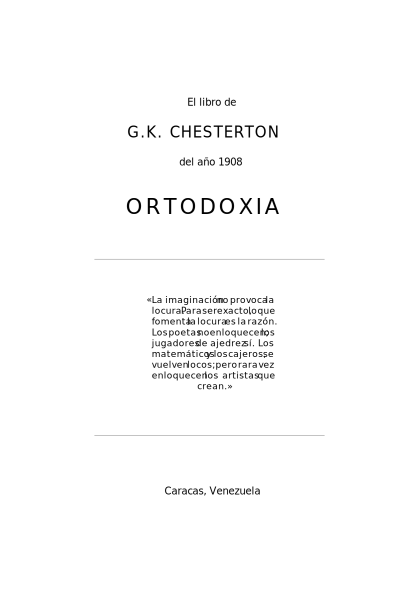
\includepdf[fitpaper=true]{portada}	
\end{titlepage}
\thispagestyle{empty}
\frontmatter
\thispagestyle{empty}
\vspace*{\fill}
\begin{small}
	\makebox[\linewidth][l]{
		\begin{tabular}[l]{rl}
	Título & Ortodoxia\\
	Autor & G.\,K. Chesterton \\	
	\addlinespace[.5em]
	Editor & Jhonny Lanzuisi\\
	email & \url{jalb97@gmail.com}\\
	Institución & Universidad Simón Bolívar\\
	\addlinespace[.5em]
	Versión de \LaTeX{} & \LaTeXe{}\\
	Motor & \LuaLaTeX
\end{tabular}
}
\end{small}

\tableofcontents
\chapter{Nota a la primera edición}

\textbf{Esta edición esta basada} en una versión digital del libro,
publicada en Argentina en 1998,
de la editorial Porrúa y presenta muchas mejoras respecto a dicha versión.

Se han añadido referencias históricas y diversas notas al margen, para
ayudar al lector dando contexto y significado a ciertos pasajes del libro.

Esta edición esta motivada por la carencia de una versión digital de calidad
y disponible a todo el público. La única versión parecida, aunque en ingles,
es la distribuida por el Proyecto Gutenberg.\nota{Este proyecto se encarga de digitalizar libros antiguos de forma gratuita, se pueden encontrar en: \url{https://www.gutenberg.org/}}

% El lector hará bien en nota que, si esta usando la versión digital de libro, las referencias a las notas al final (como la del proyecto Gutenberg en el párrafo anterior) son enlaces. Más aún, el número de la nota al final es otro enlace para regresar al texto: así se podrá reducir el tedio de buscar en cual página estaba leyendo.

\section*{Colofón}

La fuente principal es Latin Modern Roman a 10pt, Questa Grande para los títulos de los capítulos, Iwona Condensada para las notas al margen e Iosevka para los enlaces a internet y demás contenido usualmente mono-espaciado.

\chapter{Prefacio}%
\label{cha:Prefacio}

\textbf{Por extraña casualidad}, a la misma hora en que, en su vivienda campesina de Beaconsfield, fallecía
Gilbert Keith Chesterton, anunciaba George Bernard Shaw, en Newcastle, que no hablaría más en
público.

Con estos mosqueteros, que tantas veces midieron sus armas dialécticas, el espectáculo de la
refriega ideológica perdió en Inglaterra sus dos más diestros, tenaces y fantásticos combatientes.

Chesterton y Shaw nacieron tal para cual. Dotados del mismo vigor polémico e idéntico afán
proselitista, iguales en ingenio, no existía bajo el sol una sola cuestión frente a la cual sus opiniones no se
encontraran en diametral oposición.

La oposición de sus opiniones encendió y mantuvo encandilada, sin un momento de desmayo,
durante dos generaciones, la más fragorosa batalla que engendró nunca la inventiva. Sus controversias
públicas eran como justas de la razón dirimidas con los fuegos artificiales de las paradojas, las sutilezas,
los retruécanos y las imágenes, donde el público olvidaba el objeto de la riña y se dejaba fascinar por el
deslumbrante espectáculo.

Shaw vencía en el arte de la dramatización de su causa, pero Chesterton le vencía en la sutileza que
infundía al argumento de la suya.

Como si quisiera compensarle de la monstruosa corpulencia que levantó sobre sus pies, el Creador
dotó el cerebro de Chesterton con el más ágil, elástico, fino entendimiento que puso en ninguno de
nuestros contemporáneos. Era tan gigantesco y pingüe que le llamaron \textquote{monumento andante de Londres},
y en una ocasión, durante un banquete en su honor, Bernard Shaw dijo a la hora de los discursos: \textquote{Tan
galante es nuestro agasajado, señores, que esta misma mañana les dejó su asiento en el tranvía a tres
señoras}.

Fantasía o imaginación no iban a la zaga de su figura en cuanto a exuberancia.
Aunque, superficialmente considerada, la obra de Chesterton aparece sólo como un intento
ingenioso de encontrar la verdad por procedimientos originales en los que el ingenio y la originalidad
semejan lo principal y la verdad lo secundario, en realidad ocurre todo lo contrario.

Chesterton vivió perpetuamente desasosegado por la idea de la verdad, y sus paradojas no eran sino
el doble lazo con que pretendía coger por los cuernos tan elusivo toro.

Su versatilidad estaba propulsada por el mismo desasosiego, el cual le llevaba del verso al artículo
de periódico; de éste al ensayo filosófico; del ensayo a la novela teológica, cuando no detectivesca, o al
discurso proselitista y a la controversia.

La búsqueda de la verdad le condujo al catolicismo en 1922 y, poco después, a la fundación del
movimiento distributista, en el que pretendía encarnar su ideología y al que, secundado por su fiel y
veterano escudero el escritor casticista Hilaire Belloc\nota{Belloc (1870\enraya1953) fue un prolífico escritor franco-británico. Su fuerte fé católica influencia todo su trabajo. \textquote{Todo conflicto humano es, en última instancia, teológico.}}, dedicara la mayor parte de su astronómica energía
durante los diez últimos años.

Chesterton odiaba tanto al capitalismo como al comunismo, porque ambos destruyen igualmente la
propiedad privada individual, el ejercicio de los oficios manuales que, para él, constituyen la base de la
libertad y el desenvolvimiento espiritual del hombre.

En el imaginario \say{Reino distributivo} cada individuo es propietario de las herramientas con que
trabaja, ejerce su oficio individualmente y posee su vivienda. Para propulsar el triunfo del Estado
distributivo, que debe ser alcanzado por los medios constitucionales, \textquote{puesto que los ingleses aborrecen la
violencia}, Chesterton fundó un semanario, excelente y brillantemente escrito, titulado \say{G.\,K's Weekly},
es decir, \say{Semanario de Chesterton}, donde colaboraba una pléyade escogida de jóvenes intelectuales
católicos.

La concepción chestertoniana de la economía estaba íntimamente vinculada a la que tenía de la
libertad.
La libertad abstracta que la Reforma impuso sobre Europa es, según Chesterton, una maldición que
ha devorado la libertad concreta que se gozaba anteriormente en los pueblos de la Cristiandad:

\begin{quote}
La
libertad de la post-Reforma significa esto: cualquiera puede escribir un folleto, cualquiera puede dirigir un
partido, cualquiera puede imprimir un periódico, cualquiera puede fundar una secta. El resultado ha sido
que nadie posee su propia tienda o sus propias herramientas, que nadie puede beber un vaso de cerveza o
apostar a un caballo. Ahora yo les ruego a ustedes, con toda seriedad, que consideren la situación desde el
punto de vista del hombre del pueblo. ¿Cuántos seres humanos desean fundar sectas, escribir folletos o
dirigir partidos?
\end{quote}

Esta cita es un ejemplo característico del procedimiento con que Chesterton mezcla lo arbitraria y lo
lógico, el sentido común y lo absurdo para, después de fundirlos en el crisol de su imaginación, elevar el
resultado a teoría.

Tan natural como su extravagante figura física era en Chesterton la jovialidad intelectual, el gozo en
el puro juego de la inteligencia y la frase chispeante. Cualquier argumento podía ser convertido por él,
automáticamente, en un deslumbrador juego de prestidigitación.

Muchas de sus frases y de las incidencias de sus controversias se han convertido ya en leyenda que
el pueblo transmite de boca en boca. Un día debatía por la radio con un poeta defensor del verso libre,
quien le acusó de no entender la \say{nueva métrica}:

---Verso libre no es una nueva métrica, del mismo modo que dormir al
raso no es una nueva forma de arquitectura.

---Pero no podrá usted negar que es una revolución en la forma literaria.
	
---El verso libre es una revolución, respecto a la forma literaria, igual que el comer carne cruda es una
revolución respecto al arte de la cocina.

A la agudeza y mordacidad intelectual, que Ie hacían un enemigo temible, se unían en la inmensa
humanidad de Gilbert Keith una bondad y campechanía primitivas y populares que le convertían en el
más delicioso de los amigos. De su amistad privada disfrutaban muchos de aquellos con quienes
Chesterton cambiaba en público los más inflexibles mandobles: librepensadores, racionalistas,
protestantes, socialistas, eugenistas, y, especialmente, la encarnación misma de todos estos \say{ismos}, el
inescrutable, invencible, incorregible George Bernard Shaw.

Con Bernard Shaw y Lloyd George compartió Chesterton el privilegio único de que tanto en los
periódicos como en las conversaciones se le mencionara por las solas iniciales de su nombre. \textquote{¡Pobre G.\,K. Chesterton!}, se decía la gente al saludarse, en Londres, el día de su muerte.

Una de las mejores biografías que existe hoy de Bernard Shaw la escribió, en 1909, Chesterton.
Antes había escrito ya una de sus obras maestras, la biografía de poeta Browning.
Más tarde escribió las de Chaucer, Stevenson, Colbett, San Francisco de Asís y Santo Tomás de
Aquino. Dos meses antes de morir había terminado la suya propia.

Sus libros de poemas llenan casi una biblioteca. Uno de ellos se titula \emph{Bagatelas tremendas}. Las
dos novelas más famosas que escribió: \emph{El hombre que fue jueves} y \emph{El padre Brown}, están traducidas
al español, pero, en cambio, creo que no ha sido trasladado al castellano ninguno de sus últimos libros, ni
siquiera el epos de \emph{Lepanto}.

\emph{The Napoleon of Notting Hill} y \emph{A Club of Queer Trades} son novelas de la vida suburbana de
Londres, en las que revive el espíritu \say{pickwickiano}.\nota[][-17em]{\emph{Los papeles póstumos del club pickwick} es la primero novela publicada por Charles Dickens en 1836, cuyo personaje principal es Samuel Pickwick.} Chesterton hace de los personajes de sus novelas
instrumentos en que emplear su ingenio y les obliga a proceder del modo más incongruente que jamás
procedieron los habitantes del mundo novelesco.

De entre las obras teóricas o filosóficas, aparte de \emph{Ortodoxia}, aquella en que la ideología del autor
adquiere más coherencia es la contenida en el tomo de ensayos sobre el tema \emph{Qué hay de malo en el
mundo}, donde arguye contra las concepciones eugenistas,\nota[][-13em]{Y no solo contra ellas: el capitalismo y, según Chesterton sus cómplices, los socialistas reciben pocos halagos de su parte. El capítulo final de dicho libro es quizás el mejor llamado a la revolución nunca escrito, partiendo de los cabellos rojos (como el fuego) de una niña pequeña.} las cuales asumen que la suerte de la vida está
determinada por el nacimiento, y hace la más impresionante descripción del concepto cristiano de la vida
que se haya escrito en este siglo.

Aunque sostuvo siempre la opinión de que el viajar contrae la inteligencia y apoca la fantasía, visitó
Italia, Irlanda y América y escribió un libro sobre las impresiones recibidas en cada uno de dichos países.

Al revés que Bernard Shaw y Wells, las otras dos grandes figuras de las letras inglesas de su
tiempo, Chesterton no sufrió privaciones en su juventud, sino que disfrutó de la más esmerada educación
que en aquella época podía recibir un hijo de burgueses ricos.

A pesar de que era dieciocho años más joven que Bernard Shaw, sus obras comenzaron a ser
conocidas al mismo tiempo que las de éste. Chesterton no desempeñó nunca, en realidad, otra ocupación
que la de escritor, a la que se dedicó por entero desde los veinte años, después de haber abandonado el
aprendizaje de dibujante. Por entonces consistía su cultura, fundamentalmente, en un profundo
conocimiento de la Biblia que le había infundido el padre, propietario de un importante negocio de
alquileres. Por las venas de la madre corría sangre francesa.

Tuvo un solo hermano, Cecil, que se dedicó también al periodismo y había logrado gran renombre
cuando, poco después de la guerra, vino a sorprenderle la muerte.

A los veinticinco años se casó y de su matrimonio no le quedó ningún hijo a la viuda.
Su vida toda fue una portentosa exhibición de atletismo intelectual y de entusiasmo espiritual.

\begin{flushright}\small
	\addfontfeature{LetterSpace=8} AUGUSTO ASSÍA.
\end{flushright}
\finalCapituloOrnamento


\mainmatter
\chapter{Introducción en defensa de todo lo demás}%
\label{cha:Introducción en defensa de todo lo demás}

\textbf{La única justificación posible} para este libro, consiste en ser la respuesta a un desafío. Hasta un mal
tirador se dignifica aceptando un duelo.
\P~
Cuando hace algún tiempo publiqué una serie de apresurados; pero sinceros ensayos bajo el título
de \say{Heréjes}, algunos críticos por cuyas inteligencias siento caluroso respeto (puedo mencionar
especialmente al señor G.\,S. Street,\nota{George Slythe Street (1867\enraya) fue un novelista y periodista británico. Trabajaba para el \say{National Observer}, un periódico conservador apologista del imperialismo de los años de preguerra.}) dijeron que estaba muy bien de mi parte sugerir a todos que probaran
su teoría cósmica, pero que yo había evitado diligentemente confirmar mis consejos con el ejemplo. \textquote{Voy a comenzar a preocuparme por mi filosofía,} dijo el señor Street, \textquote{cuando el señor Chesterton nos haya expuesto la suya}. Tal vez fue imprudente hacer tal indicación a una persona demasiado dispuesta a
escribir libros por la provocación más leve.\nota{Chesterton no bromea: llegó a escribir mas de 170 libros, entre ellos varias recopilaciones de cuentos y artículos.} Pero después de todo, aunque el señor Street haya inspirado y
provocado la creación de este libro, no tiene ninguna necesidad de leerlo.
\P~
Si lo lee, verá que en forma personal, en sus páginas he intentado dar testimonio de la filosofía en la
cual he venido a creer, valiéndome de un conjunto de imágenes mentales más que de una serie de
deducciones. No voy a llamarla \say{mi filosofía}, porque yo No la hice. Dios y la Humanidad la hicieron; y
ella me hizo a mí.
\P~
Con frecuencia he sentido deseos de escribir una novela sobre un \say{yachtman} inglés que erró
levemente su ruta y descubrió Inglaterra convencido de haber descubierto una nueva isla en los mares del
Sur. No obstante, siempre me encontré demasiado perezoso o demasiado ocupado para escribir sobre ese
refinado tema. Por consiguiente puedo postergar una vez más mi deseo, ahora por fines de ilustración
filosófica.
\P~
Probablemente existirá la impresión general de que se sintió muy tonto el hombre que llegó a tierra
(armado hasta los dientes y hablando por señas) para plantar la bandera inglesa sobre aquél templo
bárbaro que resultó ser el Pabellón de Brighton. No me concierne a mí negar que parecía tonto. Pero si
ustedes se imaginan que se sintió tonto, por lo menos que la sensación de tontera fue su única y
dominante emoción, significa que no han estudiado con minuciosidad suficiente, la rica naturaleza
romántica del héroe de este cuento. Su error fue en verdad un error muy envidiable. Y él lo sabía, si era el
hombre que yo imagino.
\P~
¿Qué podría ser más agradable que sentir, simultáneamente y en pocos minutos, todas las
fascinadoras angustias del partir, combinadas con toda la seguridad humana de volver a casa? ¿Qué mejor
que gozar con la diversión de descubrir África, sin tener la desagradable necesidad de trasladarse a ese
continente? ¿Qué podría ser más agradable que felicitarse por descubrir Nueva Gales del Sur y
comprender luego, con lágrimas de alegría, que en realidad no era más que la vieja Gales del Sur?
Este, al menos a mi parecer, es el problema principal de los filósofos y en cierta forma, el principal
problema de este libro.
\P~
¿Cómo es posible que el mundo nos asombre y al mismo tiempo nos hallemos en él como en
nuestra casa?
¿Cómo puede este pueblo cósmico, con sus monstruos y lámparas antiguas, cómo este mundo puede
hacernos sentir simultáneamente, la fascinación de un pueblo exótico y el confort y el honor de ser
nuestro propio pueblo?
Demostrar que una creencia o una filosofía es verdadera desde todo punto de vista, sería empresa
demasiado grande aún para un libro más vasto que éste; es necesario atenerse a una sola línea de
argumentación; y esa es la táctica que me propongo observar.
\P~
Quiero dejar expuesta mi fe, como llenando esa doble necesidad espiritual: la necesidad de aliar lo
familiar con lo extraño, afiliación que con acierto el cristianismo llama \emph{romance}. Porque la misma
palabra \emph{romance}, tiene en sí el misterio y el primitivo significado de \emph{Roma}.
\P~
Cualquiera que se disponga a discutir algo, debe empezar siempre, especificando qué es lo que no
discute. Antes de determinar qué se propone probar, debería determinarse qué es lo que no se propone
probar.
\P~
Lo que no intento probar, lo que me propongo dejar como lugar común a mí y a la mayoría de los
lectores, es esta inclinación a una vida activa e imaginativa, pintoresca y llena de poética curiosidad; a
una vida como la que el hombre occidental, por lo menos aparenta haber deseado siempre.
\P~
Si un hombre opina que la extinción es mejor que la existencia o que una vida vacía y monótona es
mejor que la variación y la aventura, ese hombre no es uno de los seres normales a quienes me dirijo. Si
un hombre no tiene preferencia por nada, nada puedo darle. Pero aproximadamente todas las personas que
he encontrado en esta sociedad occidental en que vivo, estarían de acuerdo con la idea general de que
necesitamos esta vida de novela práctica; la combinación de algo que es extraño y problemático con algo
que es familiar y seguro. Necesitamos eso para vislumbrar al mundo combinando una idea de asombro
con una idea de bienvenida. Necesitamos ser felices en este mundo de maravillas sin sentirnos en él ni
siquiera confortables. Es esta enseñanza concluyente de mi credo, lo que voy a contemplar en las
siguientes páginas.
\P~
Pero tengo una razón personal para mencionar al hombre en el yacht que descubrió Inglaterra.
Porque ese hombre soy yo. Yo descubrí Inglaterra.
No sé cómo podría evitar que este libro girara en tomo al \say{ego}; y para decir verdad no sé cómo
evitar que resulte árido y confuso.
Su aridez, sin embargo, me librará del reproche que más lamento, el reproche de ser irónico y
petulante.

El sofisma liviano, es lo que más desprecio y tal vez resulte un hecho saludable que se me acuse
precisamente de usar de él. No conozco nada más despreciable que una simple paradoja; que es una
simple e ingeniosa defensa de lo indefinible. Si fuera cierto (según se ha dicho) que el señor Bernard
Shaw vivía de paradojas, el señor Bernard Shaw sería un vulgar millonario, porque un hombre de su
actividad mental, puede inventar un sofisma cada seis minutos. Inventar un sofisma es tan fácil como
mentir; porque es mentir. Lo cierto, naturalmente, es que el señor Shaw se ha visto cruelmente trabado,
por el hecho de que no puede decir una mentira, a menos que piense decir una verdad.

Yo también me siento bajo la misma intolerable trabazón. Jamás en mi vida dije nada por la sola
razón de creer gracioso lo que decía; no obstante, es claro que he tenido la vulgar vanidad humana, de
hallarlo gracioso porque yo lo había dicho.

Narrar una entrevista con una gorgona, criatura que no existe, es una cosa. Y otra cosa es descubrir
que el rinoceronte existe y deleitarse luego en el hecho de que parece que no existiera.

Se busca la verdad, pero es posible que instintivamente se persigan las verdades más increíbles, y
ofrezco este libro, con los sentimientos profundos del corazón, a la buena gente que detesta lo que escribo
y lo mira (muy justamente a mi entender) como una pobre payasada o como ejemplar de broma de mal
gusto.

Porque si este libro es una broma, es una broma contra mí mismo. Soy el hombre que haciendo
derroche de audacia, descubrió lo que ya había sido descubierto.

Si hay una sombra de farsa en lo que sigue, yo, soy el objeto de esa farsa; porque este libro explica
cómo imaginé ser el primero en poner pie en Brighton y cómo descubrí luego, que en realidad era el
último.
Cuento mis fantásticas aventuras en busca de lo evidente.

Nadie podría hallar mi caso más ridículo de lo que lo pienso yo; ningún lector puede acusarme aquí
de intentar ridiculizarlo. Yo soy el ridículo de esta historia y nadie ha de rebelarse para arrojarme de mi
trono. Confieso abiertamente todas las ambiciones de fines del siglo \textsc{xix}. Yo, como otros solemnes
chiquilines, traté de anticiparme a la época. Como ellos, intenté adelantarme por diez minutos a la verdad,
y encontré que ella se me había adelantado unos 1800 años. Esforcé la voz gritando mis verdades con
una penosa exageración juvenil, y recibí el castigo más adecuado, porque yo conservé mis verdades, pero
descubrí luego que si bien mis verdades eran verdades, mis verdades no eran mías.

Me hallé en la ridícula situación de creer que me sostenía sólo: estando en realidad sostenido por
toda la cristiandad.
Posiblemente, (y el ciclo me perdone) traté de ser original; pero sólo llegué a inventar una copia
imperfecta, de las ya existentes tradiciones de la religión civilizada. El hombre del yacht creyó descubrir
Inglaterra; yo creí descubrir Europa.

Traté de encontrar para mi uso, una herejía propia, y cuando la perfeccionaba con los últimos
toques, descubrí que no era herejía, sino simple ortodoxia.

Es posible que alguien se divierta con el relato de este chasco feliz; es posible que un amigo o un
enemigo se entretenga leyendo cómo gradualmente aprendí la verdad de una leyenda falseada o de la
falsedad de alguna filosofía difundida, cosas que pude aprender en mi catecismo. Si alguna vez lo hubiera
estudiado.

Es posible que haya diversión, o que no la haya, en leer cómo encontré al fin, en mi club anarquista
o en un templo babilónico, lo que pude encontrar en la iglesia parroquial vecina.

Si alguien se entretiene enterándose cómo las flores del campo o las frases que se oyen en el
ómnibus, o los incidentes de los políticos, o las preocupaciones de los jóvenes, se unieron en un cierto
orden para producir una cierta convicción de ortodoxia cristiana, ese alguien posiblemente pueda leer este
libro.

Pero en todo cabe una razonable división del trabajo. Yo escribí el libro, pero nada en el mundo
podría inducirme a leerlo.

Agrego una advertencia esencialmente pedante. Estos ensayos se limitan a discutir el hecho actual,
de que en el eje central de la teología cristiana (suficientemente resumida en el Símbolo de los Apóstoles)
se halla el mejor punto de apoyo para una ética enérgica y consistente.

Mis ensayos no intentan discutir el interesante, pero diferente punto de cuál es la actual sede de
autoridad que proclama ese Credo.

Aquí, el término ortodoxia, significa \say{credo de los Apóstoles} según lo entienden los que se
llamaban cristianos hasta hace muy poco tiempo y según la conducta histórica, de los que sostuvieron tal
credo.

Por razones de espacio me he visto forzado a limitarme a lo que he extractado de ese Credo; no toco
el asunto, tan discutido por los cristianos modernos, del origen del cual nosotros lo obtuvimos.

Esto no es un tratado eclesiástico, sino una autobiografía un poco deshilada.
Pero si alguno quiere saber mi opinión sobre la actual sede de autoridad de tal creencia, el señor G.\,S. Street no tiene más que arrojarme un nuevo desafío, y gustoso le escribiré otro libro.
\finalCapituloOrnamento

\chapter{El maniático}%
\label{cha:El maniático}

\textsc{ni siquiera la gente mundana} comprende al mundo; confía enteramente en unas cuantas máximas
cínicas, que no son ni verdaderas.

Recuerdo una vez: caminaba con un próspero editor que me hizo una observación oída con
frecuencia; es casi un estribillo del mundo moderno. No obstante haberla oído con demasiada frecuencia,
o tal vez por esa misma razón, recién entonces, repentinamente, vi que tal observación no entrañaba
verdad alguna. El editor dijo de alguien: \textquote{ese hombre va a llegar; se tiene fe}.

Y recuerdo que mientras levantaba la cabeza para escuchar mejor, mi mirada cayó en un ómnibus
que llevaba escrito su punto de destino: \say{Hanwell}\,\nota{Nombre de un sanatorio de enfermos mentales, que se menciona con frecuencia en el libro.} y le contesté: 

---Quiere que le diga dónde están los
hombres que se tienen fe?, porque puedo decírselo. Conozco hombres que creen en sí mismos más
colosalmente que Napoleón y César. Puedo llevarlo hasta los tronos de los superhombres. Los que
realmente se tienen fe, están en un asilo de lunáticos.

Me respondió que no obstante esa creencia mía, había muchos hombres que se tenían fe y no
estaban en manicomios.

	---Sí; los hay ---repuse---, y usted más que nadie debe conocerlos. Aquel poeta borracho a quien usted
rechazó una tragedia lúgubre creía en sí mismo. Aquel viejo pastor que escribió una obra épica y de quien
usted se escondía en la trastienda, creía en sí mismo. Si usted consultara su experiencia de editor en vez
de consultar su horrenda filosofía individualista, sabría que haberse tenido fe, es una de las características
más comunes de los fracasados. Los actores que no pueden actuar, creen en sí mismos, y creen en sí
mismos los deudores que no le pueden pagar. Sería más cierto decir que un hombre fracasará porque se
tiene fe.

	>>Tener completa fe en sí mismo, no es exclusivamente un pecado. Tenerse fe absoluta es una
debilidad. Tenerse fe completa, creer completamente en sí mismo, es tener una creencia histérica y
supersticiosa. El hombre que la tiene, lleva la palabra \say{Hanwell} escrita en su frente, con tanta claridad
como la lleva escrita ese ómnibus.

Mi amigo el editor, dio esta profunda y efectiva réplica a mis conclusiones: \textquote{Y si un hombre no debe creer en sí mismo ¿en qué debe creer?}, Luego de una larga pausa contesté, \textquote{Iré a casa y escribiré un libro contestando a esa pregunta.}

Y este es el libro que escribí para contestarla.
Pero creo, que muy bien puedo empezarlo donde se inició nuestra discusión; en la vecindad de un
manicomio.

Los modernos maestros de la ciencia insisten, sobre la necesidad de basar toda investigación, en un
hecho. Los antiguos maestros de religión, se mostraron igualmente entusiastas de esa teoría. Empezaron
basándose en el hecho del pecado; un hecho tan evidente como las papas. Fuera posible o no fuera posible
que el hombre se purificara con ciertas aguas milagrosas, no cabe duda de que necesitaba purificación.

Pero algunos caudillos religiosos de Londres, relativamente materialistas, comenzaron en nuestros días a
negar, no la discutible milagrosidad del agua, sino a negar la indiscutible existencia de la mancha. Ciertos
teólogos modernos, discuten el pecado original, que es el único punto de la teología de la cristiandad que
puede ser realmente probado. Algunos discípulos del Reverendo R.\,J. Campbell, admiten la inocencia
divina que no pueden vislumbrar ni en sueños, pero niegan, especialmente, la culpa humana que pueden
ver hasta en la calle. Los santos más intransigentes y los más obcecados escépticos, por igual unos y
otros, tomaron el positivo mal, como punto de partida de sus argumentaciones.

Si es cierto (como evidentemente lo es) que un hombre puede hallar exquisito placer desollando un
gato, el filósofo religioso puede llegar a una de dos conclusiones. Debe, o negar la existencia de Dios, que
es lo que hacen los ateos; o bien negar la inalterable unión entre Dios y el hombre, que es lo que hacen los
cristianos. Parece que los nuevos teólogos piensan llegar a una solución altamente racionalista negando el
gato.

En esta situación especialísima, evidentemente ahora no es posible (con una esperanza remota de
aceptación general) comenzar como comenzaron nuestros padres, basándose en el hecho del pecado. Este
mismo hecho que fue para ellos (y es para mí) tan evidente como la luz, es precisamente el hecho que ha
sido discutido o negado. Pero aunque los modernos nieguen la existencia del pecado, supongo que no han
negado aun la existencia del manicomio.

Todavía estamos de acuerdo en que actualmente se produce un colapso intelectual tan innegable e
inconfundible como el derrumbe de una casa. Los hombres niegan el infierno; pero aun no niegan el
manicomio. Para no perder de vista los fines de nuestro primer argumento, el uno, el infierno, podría muy
bien reemplazar al otro, el manicomio. Quiero decir que, si una vez todos los pensamientos y las teorías
fueron juzgadas según condujeran al hombre a perder su alma, así, por nuestro presente punto de vista,
todas las teorías modernas pueden ser juzgadas, según conduzcan al hombre a perder sus cabales.

Es cierto que algunos hablan de la locura, con soltura y simpatía, como si se tratara de algo amable
y atrayente.

Pero un minuto de reflexión basta para demostrarnos que si hallamos belleza en la enfermedad,
generalmente es en la enfermedad de otro.

Un ciego puede ser pintoresco; pero se necesitan dos ojos para verlo pintoresco, y similarmente,
aun la más salvaje poesía de la locura, sólo puede percibirla el cuerdo. Para el insano su locura es
perfectamente prosaica porque es perfectamente cierta. El hombre que se cree pollo, siente en sí, toda la
insignificancia del pollo. Solamente porque vemos lo grotesco de su idea, podemos en encontrarla hasta
divertida; y solamente porque él no ve lo grotesco de su idea, lo han llevado a \say{Hanwell}. Abreviando, las
rarezas sólo sorprenden a la gente normal. Las rarezas no sorprenden a la gente rara. Por esa razón, la
gente normal se sabe divertir y la gente rara, siempre se lamenta del aburrimiento de la vida. Por esa
razón, las novelas modernas fenecen; y por esa razón, los cuentos de hadas permanecen. Los viejos
cuentos de hadas presentan al héroe como un joven humano completamente normal; sus aventuras son las
sorprendentes; y lo soprenden porque es normal. Pero en la novela psicológica moderna, el héroe es un
anormal; él, que es el centro, no es bien centrado. De ahí que las aventuras más extrañas no logren
sorprenderlo adecuadamente y que el libro resulte monótono. Se puede escribir la historia de un héroe
entre dragones; pero no la de un dragón entre dragones. El cuento de hadas relata lo que hará un hombre
cuerdo en un mundo loco. La novela, sobriamente realista de hoy, relata lo que un hombre esencialmente
loco, puede hacer en un mundo cuerdo.

Empecemos pues en el manicomio; desde este fatídico y fantástico albergue, iniciemos nuestro viaje
intelectual.

Ahora, si es que vamos a contemplar la filosofía de la cordura lo primero que hemos de hacer, es
destruir un grande y difundido error. Por todas partes se ha difundido la idea de que la imaginación,
especialmente la imaginación mística, es peligrosa para el equilibrio mental del hombre. En general se
tiene a los poetas como inseguros, desde el punto de vista psicológico; y generalmente se hace asociación
de ideas entre los laureles entrelazados y las pajas pinchadas en el pelo... Los hechos y la historia
desmienten tal interpretación. Muchos de los poetas, de los verdaderamente grandes poetas, han sido no
sólo perfectamente cuerdos sino extremadamente aptos para el comercio; y si Shakespeare alguna vez
contuvo caballos, fue porque era el hombre más indicado para contenerlos.

La imaginación no provoca la locura. Para ser exacto, lo que fomenta la locura es la razón. Los
poetas no enloquecen; los jugadores de ajedrez sí. Los matemáticos y los cajeros, se vuelven locos; pero
rara vez enloquecen los artistas que crean. Como podrá verse, en ninguna forma ataco la lógica: digo
solamente que el peligro de la locura reside en la lógica; no en la imaginación. La paternidad artística es
tan saludable como la física. Sin embargo, vale la pena destacar que cuando un poeta fue realmente
mórbido, comúnmente lo fue porque existía algún punto débil de racionalismo en su cabeza. Poe, por ejemplo, fue
realmente morboso; no porque fue poético, sino porque fue esencialmente analítico. Aun el ajedrez era
demasiado poético para él; le desagradaba porque había demasiados caballeros y castillos, como en un
poema.

Abiertamente manifestó su preferencia por las fichas negras, que sobre el damero parecían el
punteado de un diagrama. Quizás el ejemplo más contundente es este: que sólo un gran poeta inglés se
volvió loco.

Cowper.\nota[][-7em]{William Cowper (1731\enraya1800) fue un poeta británico. En 1973 fue enviado a un asilo para recuperarse, pues habia intentado suicidarse despues de un periodo de ansiedad y depresión. A partir de entonces Cowper estaría siempre al borde la de locura, llegando a convencerse de que estaba destinado a la perdición eterna. Sus poemas, que escribió siempre que pasaba por un momento oscuro en su vida, podrían haber sido en efecto la razón de que conservase algo de cordura.} Y decididamente, fue llevado a la locura por la ló\-gi\-ca; por la extraña lógica de la
predestinación. La poesía no fue su enfermedad sino su remedio; la poesía, en parte conservó su salud.

Por algunos momentos, pudo olvidar el rojo y sediento infierno al que lo empujaba su horrendo
necesitarismo, entre las extendidas aguas y los lirios blancos del Duse. Cowper, fue condenado por 
John Calvin y casi fue salvado por John Gilpin\nota[][9em]{Gilpin es el personaje principal de \say{The Diverting History of John Gilpin}, historia cómica escrita por Cowper en verso.}.

En todas partes, vemos que el hombre no enloquece por soñar. Los críticos son mucho más locos
que los poetas. Homero, es bastante tranquilo y completo; son sus críticos que lo destrozan en jirones de
extravagancia. Shakespeare, fue perfectamente él mismo; sólo algunos de sus críticos descubren que
Shakespeare fue otro. Y San Juan Evangelista, no obstante haber visto en su visión muchos monstruos
extraños, no vio criatura alguna tan salvaje como uno de sus comentaristas. El hecho general es claro. La
poesía es cuerda, porque flota sin esfuerzo en un mar infinito; la razón pretende cruzar el mar infinito y
hacerlo así finito.

El resultado es la exterminación mental; como lo fue la extenuación física para el señor Holbein.
Aceptarlo todo, es un ejercicio; entenderlo todo, es un esfuerzo. Lo único que desea el poeta, es
exaltación y expansión, un mundo para explayarse.
El poeta sólo pretende entrar su cabeza en el cielo.
El lógico es el que pretende hacer entrar el cielo en su cabeza. Y es su cabeza la que revienta.

Es un detalle, pero no insignificante, que este asombroso error se halla comúnmente apoyado en una
citación tergiversada.

Todos hemos oído citar la celebrada frase de Dryden:\nota[][-9em]{John Dryden (1631\enraya1700) fue uno de los grandes poetas británicos. La cita proviene del poema satírico \say{Absalom and Achitophel} en el cual Dryden cuenta la historia bíblica de la rebelión de Absalom contra el Rey David.} \textquote{el gran genio es aliado de la locura}. Pero
Dryden no dijo que el gran genio fuera aliado de la locura. El mismo Dryden era un genio y sabía mejor.

Sería difícil encontrar un hombre más romántico y más sensato. Lo que Dryden dijo, fue esto: \textquote{El gran
sabio está frecuentemente próximo a la locura}, y eso es cierto. Es exclusivamente la gran agilidad
intelectual, la que peligra desequilibrarse. También la gente podría recordar, a qué clase de hombre se
refería Dryden. No se trataba de un visionario ajeno a este mundo como Vaughan o George Herbert.\nota{Herbert y Vaughan fueron dos poetas metafísicos del siglo \textsc{xvii}.}

Hablaba de un cínico hombre de mundo, un escéptico, un diplomático, un político práctico. Esos
hombres, ciertamente están próximos al desequilibrio. Su incesante investigar en el cerebro propio y en el
ajeno, es oficio peligroso. Siempre es peligroso para la mente penetrar la mente. Una persona espiritual
preguntó por qué decíamos \say{loco como un sombrerero}. Una persona más espiritual, podría haber
respondido que el sombrerero es loco, porque debe tomar las medidas de la cabeza humana.

Y si los grandes razonadores con frecuencia son maniáticos, es igualmente exacto que los
maniáticos son grandes razonadores.

Cuando me hallaba embarcado en una controversia con el \say{Clarion}.\nota{El \say{Clarion} era un periódico británico y socialista. Dicha polémica se describe en el libro de Chesterton \say{Controversias Blatchford} Robert Blatchford fue fundador y director del \say{Clarion}.},
sobre el tema de la voluntad
libre, el eficiente escritor señor R.\,B. Suthers dijo, que la voluntad libre, era lunatismo, porque implicaba
acciones inmotivadas, y las acciones del lunático son sin causa. No me ocupo aquí de un lapsus
desastroso para la lógica determinista. Evidentemente, si una acción, aun la acción de un lunático, puede
ser inmotivada, se acaba el determinismo.
Porque si un loco puede interrumpir la cadena de causalidad, también puede interrumpirla un
hombre aunque no sea loco. 

Pero mi objeto es destacar algo más práctico. Tal vez fuera natural que un
moderno marxista ignorara todo lo referente a la voluntad libre. Pero sería ciertamente extraño que un
marxista moderno ignorara todo lo que se refiere a los lunáticos. Lo último que se podría decir de un
lunático, es que sus acciones son inmotivadas. Si algunos actos humanos pudieran ser irreflexivamente
llamados \say{sin motivo}, esos serían los insignificantes actos del hombre cuerdo, que silba al caminar; roza
el césped con su bastón; golpea los talones y se frota las manos. Es el hombre contento el que hace las
cosas inútiles; el hombre enfermo no es bastante fuerte para ser un ocioso.

Esas acciones sin causa y descuidadas, son precisamente las que un loco no podría comprender
nunca, porque el loco (como el determinista) tiene demasiado en cuenta las causas de todo. Esas
actividades huecas, tienen para un loco significado de conspiración. Pensará que rozar el pasto, es atentar
contra la propiedad privada. Pensará que golpear los talones, es una señal convenida con un cómplice. Si
por un instante el loco se volviera descuidado, se volvería cuerdo. Todo el que haya tenido la desgracia de
hablar con gente que se hallara en el corazón o al borde del desequilibrio mental, sabe que su
característica más siniestra, es una horrible lucidez para captar el detalle; una facilidad de conectar entre
sí dos cosas perdidas en su mapa confuso como un laberinto. Si ustedes discuten con un loco, es muy
probable que lleven la peor parte en la discusión; porque en muchas formas, la mente del loco es más ágil
y rápida, al no hallarse trabada por todas las cosas que lleva aparejadas el buen discernimiento. No lo
detiene el sentido del humor o de la caridad o las ya enmudecidas certezas de la experiencia. El loco es
más lógico, por carecer de ciertas afecciones de la cordura. La frase común que se aplica a la insania,
desde este punto de vista es errónea. El loco no es el hombre que ha perdido la razón. Loco es el hombre
que ha perdido todo, menos la razón.

Las explicaciones que un loco da sobre algo son completas y con frecuencia, en un sentido
estrictamente racional, hasta son satisfactorias.
O para hablar con más precisión, la explicación del insano si bien no es concluyente, es por lo
menos irrefutable; y esto puede observarse en los dos o tres casos más comunes de locura.

Si un hombre dice (por ejemplo) que los hombres conspiran contra él, no se le puede discutir más
que diciendo que todos los hombres niegan ser conspiradores; que es exactamente lo que harían los
conspiradores. Su exposición concuerda con los hechos tanto como la de ustedes. O si un hombre dice
que es el legítimo Rey de Inglaterra, no es una respuesta adecuada decirle que las autoridades lo catalogan
loco; porque si realmente fuera Rey legítimo de Inglaterra, eso posiblemente sería lo más sabio que
atinaran a hacer las autoridades existentes. O si un hombre dice que es Jesucristo, no es una respuesta
decirle que el mundo niega su divinidad; porque el mundo niega también la divinidad de Cristo.

Sin embargo, ese hombre está equivocado. Pero si intentamos exponer su error en términos exactos,
veremos que no es tan fácil como pudimos suponerle. Tal vez lo más aproximado que podríamos hacer, es
decir esto: que su mente actúa en un círculo perfecto pero estrecho. Un círculo pequeño es tan infinito
como uno grande; pero a pesar de ser tan infinito, no es tan amplio. Del mismo modo, la explicación del
insano es tan completa como la del sano, pero no tan vasta. Una bala es redonda como el mundo, pero no
es el mundo.

Hay algo así como una amplia universalidad; y algo así como una estrecha y restringida eternidad.
Lo podemos ver en muchas religiones modernas.

Ahora, hablando externa y empíricamente, podemos decir que la más consistente e inconfundible
seña de locura, es esta combinación entre la integridad lógica y la contracción espiritual. La teoría del
lunático, explica un vasto número de cosas, pero no explica esas cosas en forma vasta. Quiero decir que si
ustedes, o yo lidiáramos con una mente que se vuelve mórbida, lo indicado sería, no tanto ofrecerle
argumentos como darle aire, para convencerla de que existe algo más limpio y fresco, fuera de la
sofocación de un único argumento. Supongamos que fuera, por ejemplo, el primer caso típico que
mencioné: el caso de un hombre que acusara a todo el mundo de conspirar contra él. Si pudiéramos
expresar nuestros profundos sentimientos de protesta, apelando contra tal obsesión, supongo que le
diríamos algo así: \textquote{Oh; admito que usted tiene su caso y que lo siente de corazón, y que muchas cosas son
como usted dice. Admito que su explicación explica muchas cosas, pero ¡cuántas cosas no explica! ¿No
hay en el mundo más historia que la suya; y todos los hombres se ocupan de usted? Suponga que demos
por sabido los detalles; tal vez cuando aquel hombre en la calle se hizo el que no lo veía, fue por astucia;
tal vez si el agente le preguntó su nombre, lo hizo porque ya lo sabía. Pero ¡cuánto más contento estaría si
le constara que esa gente no se ocupa en absoluto de usted! ¡Cuánto más grande sería su vida si usted se
empequeñeciera en ella! ¡Si pudiera mirar a los otros hombres con curiosidad y gusto comunes, si pudiera
verlos paseando como pasean su radiante egoísmo y su varonil indiferencia! Comenzarían a interesarlo
porque vería que no se interesan en usted. Se evadiría de ese teatro vistoso y mezquino en el que siempre
se representa su dramita personal, y se encontraría bajo un cielo más despejado, en una calle llena de
espléndidos desconocidos.}

O supongamos que fuera el segundo caso de locura, el del hombre que reclama la corona; el
impulso de ustedes, sería contestarle: \textquote{Está bien; tal vez usted sepa que es el Rey de Inglaterra pero, ¿por
qué se preocupa? Haga un esfuerzo magnífico, sea un ser humano y mire de arriba a todos los reyes de la
tierra.}

O podría ser el tercer caso, del loco que se cree Cristo. Si dijéramos lo que sentimos, diríamos:
\textquote{¡Así que usted es el Creador y el Redentor del mundo! ¡Pero qué mundo pequeño debe ser! Qué cielo
más pequeño debe habitar con ángeles no tan grandes como mariposas. ¡Qué aburrido ser Dios! ¡Y un
Dios inadecuado! Realmente, no hay vida más plena ni amor más maravilloso que el suyo; y en realidad ¿es en su
mezquina y penosa compasión que toda carne debe depositar su fe? ¡Cuánto más feliz sería si la masa de
un Dios más grande, pudiera deshacer su pequeño cosmos, desparramara las estrellas como si fueran
pajas, y lo dejara en la inmensidad abierta, libre como otros hombres de mirar hacia arriba y hacia abajo!}

Y hay que recordar que la ciencia más puramente práctica, ataca desde este punto de vista al mal
mental; no intenta discutirlo como una herejía sino simplemente quebrarlo como un encantamiento. Ni la
ciencia moderna ni la religión antigua creen en la completa libertad del pensamiento. La teología reprime
ciertos pensamientos que llama blasfemos. La ciencia reprime ciertos pensamientos que llama morbosos.

Por ejemplo, algunas sociedades religiosas, más o menos exitosamente quieren alejar al hombre del
pensamiento sexual. La nueva sociedad científica, intenta alejarlo del pensamiento de la muerte; que es un
hecho, pero es considerado como un hecho morboso.

Y atendiendo a aquellos cuya morbosidad tiene un dejo de manía, la ciencia moderna se preocupa
de la lógica, mucho menos que un derviche en pleno baile. En esos casos, no es suficiente que el hombre
desgraciado desee la verdad; debe desear la salud. Nada puede salvarlo excepto una ciega ansiedad de
normalidad. Ningún hombre debe creerse a salvo del desequilibrio mental; porque es el órgano que actúa
el pensamiento el que se vuelve enfermo; ingobernable, como si fuera independiente. Sólo puede salvarlo
la voluntad o la fe. Desde que empieza a actuar su razón, actúa en la antigua ruta circular; girará en torno
de su círculo lógico, igual que un hombre en un coche de tercera clase de Juner Circle, girará en torno de
Juner Circle, hasta que realice el voluntario, vigoroso y místico acto, de bajarse en Gower Street. Aquí, la
decisión lo es todo; una puerta debe cerrarse para siempre. Cada remedio, es un remedio desesperado.

Cada cura, es una cura milagrosa. Curar a un hombre no es discutir con un filósofo, es arrojar un
demonio. Y por apaciblemente que trabajen en el asunto los doctores y los filósofos, su actitud es
profundamente incomprensiva. Su actitud es ésta: que el hombre debe dejar de pensar, si quiere seguir
viviendo. Tal tratamiento, es una amputación intelectual.

Si tu cabeza te perturba, córtatela; porque es mejor entrar al Reino de los Cielos no solamente como
un niño sino como un imbécil, que ser arrojado con la inteligencia al infierno\ldots\ o a \say{Hanwell}.

Tal es el loco de los experimentos. Por lo general es un razonador; y con frecuencia un razonador
acertado. Sin duda se le podrá derrotar en un terreno puramente racional planteándole su caso con lógica.

Pero se le puede plantear con mayor precisión en términos más generales y aún más estéticos. Está
encerrado en la pulcra y lúcida prisión de una sola idea; se ha aguzado hasta un penoso extremo. Carece
de la indecisión del sano y de su complejidad. Ahora, según expliqué en la introducción, me propongo
ofrecer en estos primeros capítulos, no tanto el diagrama de una doctrina, cuanto algunas imágenes de un
punto de vista. Y he sido extenso describiendo mi visión del maniático, por esta razón: porque así como
me impresiona el maniático, así me impresionan muchos pensadores modernos.

Esa inconfundible nota que me llega de \say{Hanwell}, la escucho también de muchas cátedras de
Ciencia y de muchas aulas de hoy día; y muchos médicos de alienados, tienen de alienados algo más que
su especialidad.

En todos se manifiesta esa combinación que hemos notado: la combinación de una razón expansiva
y extenuante, con un sentido común contraído y restringido. Son universales en cuanto se aferran a una
explicación razonable y la llevan hasta muy lejos. Pero una muestra, puede prolongarse hasta siempre y
ser no obstante, una pequeña muestra.

En un tablero de ajedrez, ven el blanco sobre el negro; si el universo entero está pavimentado como
el tablero, siempre siguen viendo el blanco sobre el negro. Como el lunático, no pueden alterar su punto
de vista; no pueden hacer un esfuerzo mental y repentinamente verlo negro sobre blanco.

Tomen primero el caso más obvio del materialismo. Para dar una explicación del mundo, el
materialismo tiene una especie de simplicidad insana.

Tiene justo la cualidad del argumento del loco; nos hace sentir simultáneamente, que todo lo abarca
y que todo lo deja afuera.

Contemplen un materialista sincero v eficiente como por ejemplo Mac Cabe, y tendrán esa exacta y
exclusiva sensación. Lo comprende todo; y todo parece no merecer la pena de ser comprendido.

Sus cosmos, puede ser completo en cada remache y en cada engranaje, pero aún así, su cosmos es
más pequeño que nuestro mundo. En cierta forma, su plan, como el lúcido plan del loco, parece insensible
a las remotas energías y a la completa indiferencia de la tierra; es no pensar en las realidades de la tierra:
en los pueblos que luchan, en las madres, en el primer amor y en el terror extendido sobre el mar. La
tierra es tan vasta y el cosmos tan pequeño. El cosmos es, algo así como el agujero más pequeño en el
cual un hombre puede esconder su cabeza.

Hay que entender que ahora no discuto la relación de esas creencias con la verdad, sino, por el
momento, solamente sus relaciones con la salud. Más compenetrados con el argumento, espero atacar el
punto de la verdad objetiva; aquí sólo hablo de un fenómeno psicológico.

Por ahora, no intento probarle a Haeckel que el materialismo es falso, como no intenté probarle al
hombre que se creía Cristo, que elaboraba sobre una creencia errónea. Aquí, destaco exclusivamente el
hecho de que ambos casos son en un mismo sentido completos, y en un mismo sentido incompletos. Se
puede explicar que la indiferencia pública detiene en \say{Hanwell} a un hombre diciendo que esa detención
es la crucifixión de un Dios que el mundo no merecía. La explicación explica. Similarmente se puede
explicar el orden universal, diciendo que todas las cosas, aún las almas de los hombres, son hojas
inevitablemente distribuidas en un árbol por completo inconsciente, i ciego destino de la materia. La
explicación explica, a pesar de no explicar tan completamente como la explicación del loco. Pero aquí el
asunto es que la mente humana normal, no sólo objeta a ambas explicaciones, sino que tiene para las dos
la misma objeción. Su testimonio aproximado es éste: que si el hombre de Hanwell es el verdadero Dios,
no tiene aspecto de serlo. Y similarmente, que si el cosmos del materialista es el verdadero cosmos no
tiene aspecto de cosmos. La cosa se empequeñece. La deidad es menos divina que varios hombres; y
(según Haeckel) el conjunto de la vida, es algo mucho más trivial, gris y estrecho, que varios aspectos
aislados de ella. Las partes parecen mayor que el todo. Porque debemos recordar que la filosofía
materialista, sea o no sea verdadera, tiene por cierto muchas más limitaciones que cualquier religión. En
un sentido por supuesto, todas las ideas inteligentes son limitadas. No pueden ser más vastas que sí
mismas. Un Cristiano está restringido solamente en el sentido en que está restringido un ateo. No puede
pensar que el Cristianismo es falso y seguir siendo cristiano; y el ateo no puede pensar que el ateísmo es
falso y seguir siendo ateo.

Pero siendo las cosas como son, hay un aspecto especial en el cual el materialismo tiene más
restricciones que el espiritualismo. El señor Mac Cabe piensa que soy un esclavo porque no me es
permitido creer en el determinismo. Creo que el señor Mac Cabe es un esclavo porque no le está
permitido creer en las hadas. Pero si examinamos las dos prohibiciones, veremos que la suya es mucho
más absoluta que la mía. El cristiano es muy libre de creer que en el mundo hay un conjunto de
ordenamientos establecidos y de sucesos inevitables. Pero el materialista no puede aceptar ni el más
mínimo dejo de espiritualismo o de milagro.

Al pobre señor Mac Cabe, no le está permitido admitir la posibilidad de que exista un geniecillo ni
escondido en una flor. El cristiano admite que el universo es variado y aún mezclado, tal como el hombre
cuerdo admite su propia complejidad. El hombre cuerdo sabe que tiene un poco de bestia, un poco de
demonio, un poco de santo y un poco de ciudadano. Y lo que es más, el hombre realmente cuerdo, admite
tener, sabe que tiene, algo de loco. Pero el mundo materialista es muy sólido y simple, así como el loco,
está completamente seguro de ser cuerdo. El materialista está seguro de que la historia es simplemente y
solamente una cadena de casualidades, así como la interesante persona que se mencionó antes, está segura
de ser simplemente y solamente un pollo. Los materialistas y los locos, nunca tienen dudas.

Las doctrinas espirituales, actualmente no limitan la mente tanto como las negaciones materialistas.

Aun creyendo en la inmortalidad, no necesito pensar en ella. Pero si no creo en la inmortalidad, no debo
pensar en ella. En el primer caso la ruta está abierta y puedo llegar tan lejos como quiera. En el segundo,
la ruta está cerrada.

Pero el caso es aún más concluyente y el paralelo con la locura, más extraño todavía. Porque
nuestro caso era contra la agotadora y lógica teoría del lunático, que bien o mal, destruía gradualmente su
humanidad. Ahora el cargo es contra las principales deducciones del materialista, que bien o mal,
gradualmente destruyen su humanidad; no me refiero sólo a la bondad, me refiero a la esperanza, al valor,
a la poesía, a la iniciativa y a todo lo que es humano. Siendo el materialismo lo que conduce al hombre
hacia el fatalismo completo (como generalmente ocurre) es inútil pretender que se trate en ningún sentido
de una fuerza libertadora. Es absurdo decir que avanza especialmente la liberación, cuando el libre
pensamiento sólo se usa para destruir la voluntad libre. Los deterministas atan, no desatan.

A su ley, bien pueden llamarla \say{cadena} de causalidad. Es la peor cadena que puede aprisionar al
ser humano. Si gustan, pueden usar el lenguaje de la libertad en la enseñanza materialista, pero salta a la
vista que tal lenguaje es en ese uso tan, pueden decir que el hombre empleara para conversar con el
hombre encerrado en el manicomio. Si gustan, pueden decir que el hombre es libre de pensar que es un
huevo hervido. Pero seguramente es de más peso e importancia el hecho, de que si es un huevo hervido,
no es libre de comer, beber, dormir, caminar o fumarse un cigarrillo.

Si gustan, igualmente pueden decir que el audaz especulador determinista es libre de no creer en la
voluntad libre. Pero en tal caso, es de mucho más peso e importancia el hecho, de que no es libre de
alabar, de maldecir, de agradecer, de justificar, de discutir, de castigar, de resistir a la tentación, de agitar
muchedumbres, de perdonar pecadores, de reprimir tiranos, o aún de decir \textquote{gracias, por la mostaza}.
Pasando de este asunto, puedo destacar que existe una extraña mistificación que presenta al
fatalismo materialista en cierta manera favorable al perdón, a la abolición de los castigos crueles o de
cualquier clase de castigo. Esto es sorprendentemente opuesto a la verdad. Es muy admisible que la
doctrina necesitarista no hace diferencias, que deja azotando al que azota y al buen amigo exhortando
como antes. Pero evidentemente que si algo detuviera, detendría la exhortación. Que los pecados sean
inevitables, no es un hecho que impide el castigo; si algo impide es la persuasión. Es tan probable que el
determinismo conduzca a la crueldad como a la cobardía. El determinismo no es incompatible con el
hecho de tratar cruelmente a los criminales. Con lo que tal vez es incompatible es con darles tratamiento
benigno; con apelar a sus mejores sentimientos; con alentarlos en su lucha moral.

El determinismo no cree en la eficacia de apelar a la voluntad, pero cree en la eficacia de cambiar el
medio ambiente. No dirá al pecador: \textquote{Ve, y no peques más}, porque el pecador no puede rehuir la ofensa.

Pero puede sumergirlo en aceite hirviendo; porque el aceite hirviendo es un medio ambiente. De ahí que
el materialista, considerado como una silueta, tenga los contornos fantásticos de la silueta del loco.

Ambos asumen una actitud, al mismo tiempo inapelable e intolerable.

Por supuesto, que todo lo que antecede se puede decir no sólo del materialista. Lo mismo podría
aplicarse al extremo opuesto de la lógica especulativa. Hay un escéptico mucho más terrible que el que
cree que todo comenzó en la materia. Es posible encontrar el escéptico que cree que todo comienza en sí
mismo. Él no duda de la existencia de los ángeles o de los demonios, sino de la de los hombres y las
vacas. Para ése, sus propios amigos no son sino una mitología hecha por él. Creó su propio padre y su
propia madre. Esta fantasía horrenda tiene algo decididamente atrayente para el egoísmo en cierta forma
místico de nuestros días. Aquel editor que pensaba que los hombres que se tenían fe, llegarían; esos
buscadores del superhombre que siempre creen encontrarlo mirándose al espejo; esos escritores que
hablan de imprimir su personalidad en vez de crear vida para el mundo, toda esa gente está realmente a
una cuarta de aquella vaciedad horrible.

Entonces, cuando en torno al hombre el mundo se haya oscurecido como una mentira, cuando los
amigos se desvanezca en espíritus y vacilen los cimientos de la tierra; entonces, cuando no creyendo en
nada y en nadie el hombre se encuentre a solas en su pesadilla, entonces el gran lema individualista se
trazará sobre él como una ironía vengadora. Las estrellas apenas serán puntos en la oscuridad de su propio
cerebro; el rostro de la madre sólo será un ensayo de su lápiz loco en las paredes del calabozo. Pero sobre
la puerta de su celda se habrá escrito con horrible verdad: \say{Cree en sí mismo.}
No obstante, lo única que nos concierne aquí, es destacar que este extremo del pensamiento egoísta,
encierra y exhibe la misma paradoja que el otro extremo del materialismo. En teoría es igualmente
completo e igualmente lisiado en la práctica. En bien de la claridad, es más fácil exponer la idea diciendo
que un hombre puede creer que siempre vive en un sueño. Pero evidentemente no se le puede ofrecer una
prueba positiva de que no sueña por la sencilla razón de que no hay prueba que no se le pueda ofrecer
igualmente mientras está soñando. Pero si el hombre comienza a incendiar Londres y dice que el ama de
llaves pronto lo llamará a tomar el desayuno, lo tomaríamos y lo llevaríamos con otros lógicos a un lugar
que se ha mencionado con frecuencia en el transcurso de este capítulo.

El hombre que no puede creer a sus sentidos y el hombre que no puede creer en nada, son
igualmente insanos, pero no es posible probar el desequilibrio por un error de sus argumentos sino por la
manifiesta equivocación conjunta de sus vidas. Ambos se han encerrado en sendas cajas pintadas
interiormente con el sol y las estrellas; los dos son incapaces de salir, uno a la salud y la dicha del cielo,
otro a la salud y la dicha de la tierra. Su posición es muy razonable; y aún más, en cierto sentido es
infinitamente razonable, así como una moneda de diez centavos es infinitamente redonda. Pero hay algo
así como una infinidad mezquina, una humillada y esclavizada eternidad. Es entretenido advertir que
muchos místicos o escépticos modernos, han tomado como insignia un símbolo oriental, que es muy el
símbolo de esta nulidad extrema. Representan la eternidad por una serpiente con la cola en la boca. Hay
un admirable sarcasmo en esta imagen de una comida poco satisfactoria. La eternidad del materialismo
fatalista, la eternidad de los teósofos arrogantes y de los científicos encumbrados de hoy, está bien
representada por la serpiente que se come la cola; un animal degradado que destruye hasta su propio ser.

Este capítulo es puramente práctico y se refiere al principal signo y elemento actual de la insania,
que es, en resumen, la razón usada sin base; la razón en el vacío. El hombre que comienza a pensar sin la
base de un primer principio adecuado, enloquece; es el hombre que empieza por el mal lado. Y en las
páginas que siguen tenemos que tratar de descubrir cuál es el buen extremo. Pero podemos preguntar, a
guisa de conclusión, si esto es lo que vuelve loro al hombre ¿qué es lo que lo conserva cuerdo?
Hacia el fin de este libro espero dar una respuesta concluyente (algunos pensarán que una respuesta
demasiado concluyente). Mas por el momento, y en la misma forma netamente práctica, es posible dar
una respuesta referente a lo que en la actual historia de la humanidad, puede conservar cuerdos a los
hombres. Mientras tienen misterios, tienen salud; cuando se destruye el misterio, se crea la morbosidad.

El hombre común siempre ha sido cuerdo, porque el hombre común siempre ha sido místico. Siempre ha
aceptado la nebulosidad. Siempre ha tenido un pie en la tierra y otro en el país de las hadas. Siempre ha
conservado la libertad de dudar de sus dioses; pero (contrariamente a los agnósticos de hoy) también ha
conservado su libertad de creer en ellos. Siempre se ha preocupado más de la verdad que de la
consistencia. Si vio dos verdades que se contradecían mutuamente, tomó las verdades y la contradicción
junto con ellas. Su vista espiritual es estereoscópica, como su vista física. Al mismo tiempo ve dos cosas
diferentes, y no obstante, o por lo mismo, las ve mejor.

De ahí que siempre haya existido algo como el destino, pero también algo como la libertad de
albedrío. De ahí que creyó que de los niños era el reino de los cielos, y que no obstante lo cual, debían
obedecer en el reino de la tierra. Admiró a la juventud porque era joven y a la vejez porque no lo era.

Es, precisamente este don de asociar las aparentes contradicciones, lo que constituye toda la
elasticidad del hombre sano. El único secreto del misticismo es éste: que el hombre puede entenderlo todo
merced a la ayuda de todo lo que no entiende. El lógico mórbido, intenta dilucidarlo todo y sólo consigue
volverlo todo misterio. El místico permite que algo sea misterioso, y todo lo demás se vuelve lúcido. El
determinista hace muy clara la teoría de causalidad y luego descubre que no puede decir \say{por favor} a la
mucama. El Cristiano acepta que la libertad de albedrío siga siendo un misterio sagrado; por eso sus
relaciones con la mucama son de una cristalina y luminosa claridad. Pone la simiente del dogma en una
oscuridad central; pero la simiente germina y se ramifica en todas direcciones con espontánea y saludable
abundancia. Así como hemos tomado al círculo como símbolo de la razón y de la locura, muy bien
podemos tomar a la cruz como símbolo al mismo tiempo de la salud y del misterio. El budismo es
centrípeto pero el Cristianismo centrífugo: se vuelca hacia afuera. Porque el círculo es perfecto e infinito
en su naturaleza; pero se halla siempre limitado a su tamaño; nunca puede ser mayor ni más pequeño.

Pero la cruz, pese a tener en su centro una fusión y una contradicción, puede prolongar hasta siempre sus
cuatro brazos, sin alterar su estructura.

Puede agrandarse sin cambiar nunca, porque en su centro yace una paradoja. El círculo vuelve sobre
sí mismo y está cernido.

La cruz abre sus brazos a los cuatro vientos; es el indicador de los viajeros libres.

Hablando de este profundo tema, los símbolos escuetos son de un valor confuso; y otro símbolo
tomado de la naturaleza expresará con claridad suficiente, lo que es el misticismo para la raza humana.

La única cosa creada que no podemos ver, es la única cosa a cuya luz podemos verlo todo. Como el
sol en su ocaso, el misticismo explica todo lo demás con los rayos de su invisibilidad victoriosa.

El intelectualismo desinteresado es (en el exacto sentido del dicho popular) puro brillo de luna,
porque es luz sin calor y luz reflejada de un mundo muerto. Pero los griegos tenían razón cuando hicieron
a Apolo dios de la imaginación y de la sensatez. Luego hablaré de los dogmas de necesidad y de un credo
especial. Pero ese trascendentalismo según el cual viven los hombres, originariamente tiene mucho de la
posición del sol en el cielo. Tenemos conciencia de él, como de una especie.
\finalCapituloOrnamento

\chapter{El suicidio del pensamiento}%
\label{cha:El suicidio del pensamiento}

\textsc{las frases callejeras} no solamente son vigorosas, sino también sutiles: porque una figura de
lenguaje con frecuencia puede llegar a ser demasiado simple para prestarse a definición. Frases como
\say{fuera de uso}, o \say{fuera de tono}, podrían haber sido acuñadas por el señor Henry James,\nota{Henry James (1843\enraya1916) fue un escritor británico considerado como uno de los mejores novelistas de la literatura inglesa} en una agonía
de precisión verbal. Y no hay verdad tan sutil como aquella de la cotidiana frase sobre el hombre que
tiene el corazón bien puesto. Abarca una idea de proporción normal; no sólo existe una cierta función,
sino que también esa función está correctamente relacionada con otras funciones. Por cierto que lo
opuesto de esa frase, describiría con gran exactitud, la piedad y la ternura, en cierta forma morbos, de los
modernos más representativas. Si por ejemplo tuviera que describir con sinceridad el carácter del señor
Bernard Shaw, no podría expresarme más exactamente que diciendo que, posee un corazón generoso y
heroicamente amplio, pero no es un corazón bien puesto. Y eso mismo ocurre con la sociedad típica de
nuestro tiempo.

El mundo moderno no es malo; en cierto modo el mundo moderno es demasiado bueno. Está lleno
de feroces y malgastadas virtudes. Cuando se perjudica una empresa religiosa (como se perjudicó el
Cristianismo con la Reforma) no es solamente de confusión espléndida; es algo brillante y sin forma, al
mismo tiempo llamarada y mancha. Pero el círculo de la luna es tan claro e inconfundible, tan periódico e
inevitable como el círculo de Euclides sobre un pizarrón. Porque la luna es completamente razonable; es
la madre de los lunáticos, y a todos ellos les ha dado su nombre.

A causa de los vicios desencadenados. Los vicios, por cierto se desencadenan y se extienden y
causan perjuicios. Pero las virtudes también andan desencadenadas; y las virtudes se extienden más
desenfrenadas y causan perjuicios más terribles. El mundo moderno está lleno de viejas virtudes cristianas
que se volvieron locas. Enloquecieron las virtudes porque fueron aisladas unas de otras y vagan por el
mundo solitarias.

De ahí que algunos cientistas se preocupan por la verdad; y su verdad es despiadada, y de allí que
algunos humanistas se preocupan sólo de la piedad y su piedad (lamento decirlo) frecuentemente es
falseada. Por ejemplo: el señor Blatchford ataca al cristianismo porque está loco por una virtud cristiana;
la puramente mística y casi irracional virtud de la caridad. Tiene la extraña idea de que facilitará el perdón
de los pecados, diciendo que no hay pecados que perdonar. El señor Blatchford es no solamente uno de
los primeros cristianos; es el único de los primeros cristianos que realmente mereció ser comido por los
leones. Porque en su caso, la acusación pagana es verdadera: su misericordia significa anarquía. En
realidad, por ser tan humano, es enemigo de la raza humana. Como extremo opuesto podríamos tomar al
realista agriado, que deliberadamente mató en sí todo placer humano, con fábulas alegres o con el
endurecimiento del corazón. Torquemada, torturaba físicamente a la gente, en bien de la verdad moral.

Zola tortura a la gente moralmente, en bien de la verdad física. Pero en tiempos de Torquemada, por lo
menos existía un sistema que hasta cierto punto permitía que la rectitud y la paz se besaran. Ahora, ambas
no se saludan ni con una inclinación de cabeza.

Pero podríamos encontrar un caso mucho más concluyente que estos dos de la piedad y de la
verdad, en la sorprendente dislocación de la humanidad.

Aquí sólo nos concierne tratar de un aspecto de la humildad. Por mucho tiempo, humildad ha
significado una restricción de la arrogancia e infinitud del apetito del hombre. Del hombre que siempre
estaba aventajando a sus misericordias con el continuado invento de necesidades nuevas.

Su propia capacidad de goce destruía la mitad de sus goces. Procurándose placeres, perdió el placer
principal; porque el principal placer es la sorpresa. De ahí resulta evidente que si el hombre quiere hacer
amplio a su mundo, él debe estar siempre haciéndose pequeño. Aún las ciudades más encumbradas y los
pináculos inclinados por su propia altura, son creaciones de la humildad. Los gigantes que derriban
montes como si fueran pasto, son creaciones de la humildad. Las torres que se pierden en lo alto por
encima de la estrella más solitaria en su lejanía, son creaciones de la humildad. Porque las torres no son
altas sino cuando las miramos desde abajo; y los gigantes no son gigantes sino más grandes que nosotros.

Toda esa imaginación de lo gigantesco, que es quizá el más vigoroso de los placeres del hombre, en el
fondo es enteramente humilde. Sin humildad es imposible gozar de nada; ni aun de la soberbia.

Pero lo que nos hace padecer el presente es la modestia mal ubicada. La modestia se ha mudado del
órgano de la ambición. La modestia se ha instalado en el órgano de la convicción: la cual nunca se la
había destinado.

El hombre estaba destinado a dudar de sí; pero no de la verdad; ha sucedido precisamente lo
contrario.

Actualmente la parte del hombre que el hombre proclama, es exactamente la parte que no debía
proclamar: su propio yo. La parte que pone en duda, es exactamente la parte de la cual no debía dudar: la
razón Divina. Huxley, predicó una humildad que se conformaba con aprender de la naturaleza. Pero el
escéptico de nuevo cuño es tan humilde, que duda hasta de poder aprender. De ahí resulta que si nos
hubiéramos apresurado a decir que no existe una humildad típica de nuestro tiempo, nos hubiéramos
equivocado. La verdad es que hay una real humildad típica de nuestro tiempo. Pero ocurre que,
prácticamente, es una humildad tan envenenada como la más desorbitada de las postraciones del asceta.

La vieja humildad era una espuela que impedía al hombre detenerse; no un clavo en su zapato que le
impedía proseguir. Porque la vieja humildad hacía que el hombre dudara de su esfuerzo, lo cual lo
conducía a trabajar más duro. Pero la nueva humildad hace que el hombre dude de su meta, lo cual lo
conduce a cesar su esfuerzo por completo.

En cualquier esquina podemos encontrar un hombre pregonando la frenética y blasfema confesión
de que puede estar equivocado. Cada día nos cruzamos con alguno que dice, que, por supuesto, su teoría
puede no ser la cierta.

Por supuesto, su teoría debe ser la cierta, o de lo contrario, no sería su teoría. Estamos en camino de
producir una raza de hombres mentalmente demasiado modestos para creer en la tabla de multiplicar. Nos
hallamos en peligro de ver filósofos que duden de la ley de gravedad, por considerarla como un simple
producto de sus imaginaciones. Los farsantes de otros tiempos eran demasiado orgullosos para dejarse
convencer; pero éstos son demasiado humildes para poder ser convencidos. Los humildes heredan la
tierra; pero los escépticos modernos son demasiado humildes, hasta para reclamar su herencia. Y
precisamente esta impotencia intelectual es nuestro segundo problema.

El último capítulo se refería a un hecho observado: que el peligro de morbidez que puede correr un
hombre, proviene más de su corazón que de su imaginación. No se intentaba atacar la autoridad de la
razón; su objeto más bien fue defenderla; porque necesita defensa.

Todo el mundo moderno está en guerra con la razón; y la torre, ya vacila.

Con frecuencia se dice que los sensatos no hallan respuesta para el enigma de la religión. Pero la
dificultad con nuestros sensatos, no es que no puedan ver la respuesta, sino que no pueden ver ni siquiera
el enigma. Son como niños suficientemente estúpidos como para no notar nada paradójico en la
manifestación de que una puerta no es una puerta. Los tolerantes modernos, por ejemplo, hablan sobre la
autoridad religiosa, no solamente como si no hubiera razón alguna de su existencia, sino como si nunca
hubiera habido una razón para que exista.

A más de no ver su base filosófica, no pueden siquiera ver su causa histórica. La autoridad religiosa,
ha sido con frecuencia opresiva e irrazonable, tal como cada sistema legislativo (y especialmente el
nuestro actual) ha sido duro y culpable de una penosa apatía. Es razonable atacar a la policía; también es
glorioso. Pero los modernos críticos de la autoridad religiosa, son como hombres que atacaran a la policía,
sin nunca haber oído hablar de asaltantes. Porque existe un grande y posible peligro para la mente
humana; un peligro tan real como el de un asalto. Contra él, bien o mal, la autoridad Religiosa se irguió
como una barrera. Y contra él, algo por cierto debe erguirse como barrera si es que nuestra raza debe
salvarse de la ruina.

Ese peligro consiste en que el intelecto humano es libre de autodestruirse. Tal como una generación
podría impedir la existencia de la generación siguiente, recluyéndose toda en monasterios o arrojándose al
mar; así un núcleo de pensadores puede impedir, hasta cierto punto, los pensamientos subsiguientes,
enseñando a la nueva generación que no existe validez en ningún pensamiento humano. Sería cargoso
hablar siempre de la alternativa entre la razón o la fe. La razón en sí misma es un objeto de la fe. Es un
acto de fe afirmar que nuestro pensamiento no tiene relación alguna con la realidad.

Si usted es puramente un escéptico, tarde o temprano se hará esta pregunta: ¿Por qué todo puede
andar bien, aun la observación y la deducción? ¿Por qué la buena lógica es tan engañosa como la mala
lógica? ¿Ambas son actividades en el cerebro de un mono sorprendido?
Hay un pensamiento que detiene el pensamiento. Y ese es el único pensamiento que debería ser
detenido. Ese es el mal concluyente contra el cual se dirigió toda la autoridad religiosa. Recién aparece al
final de edades decadentes como la nuestra; y el señor H.\,G. Wells,\nota[][-8em]{Herbert George Wells (1866\enraya1946) fue un escritor británico cuyas obras abarcan desde novelas hasta la crítica social y la sátira. Ateo y socialista, Wells abogó por la paz y trabajó en textos fundacionales de la liga de las naciones (el precursor fallido de la \textsc{onu}).} ya izó su estridente bandera; ha
escrito una delicada pieza de escepticismo llamada \emph{Las dudas del instrumento}. Allí interroga al cerebro
e intenta excluir la realidad, hasta de sus propias afirmaciones, pasadas, presentes y por venir. Contra esta
ruina lejana, se organizó y se jerarquizó originariamente, todo el sistema militar de la religión. Las
creencias y las cruzadas, las jerarquías y las persecuciones, no fueron organizadas según la ignorancia para suprimir la razón.

El hombre, por un instinto ciego sabía que si las cosas fueron discutidas
ensañadamente, la razón pudo ser discutida primero. La autoridad para absolver que tienen los sacerdotes;
la autoridad de los papas para determinar autoridades; aun la autoridad para aterrar de los inquisidores,
eran solamente sombrías defensas erigidas en torno de una autoridad central más indemostrable, más
sobrenatural que todas: la autoridad para pensar que tiene el hombre. Sabemos ahora que las cosas son
así; no tenemos excusa para ignorarlo. Porque a través de la vieja rueda de autoridades, podemos oír al
escepticismo crujiente, y al mismo tiempo ver a la razón íntegra y fuerte sobre su trono.

En tanto que la religión marche, la razón marcha. Porque ambas son de la misma primitiva y
autoritaria especie. Ambas son métodos que prueban y no pueden ser probados. Y en la acción de destruir
la idea de la autoridad divina, hemos destruido sobradamente la idea de esa autoridad humana, por la cual
podemos abreviar una división muy larga. Con un rudo y sostenido tiroteo, hemos querido quitar la mitra
al hombre pontificio, y junto con la mitra le arrebatamos la cabeza.

A menos que a esto se le llame divagación, tal vez fuera conveniente repasar rápidamente, los
principales modos de pensar modernos, que han causado este efecto de detener el pensamiento. Tuvieron
ese efecto el materialismo y la teoría de que todo es producto de una ilusión individual; porque si la mente
es mecánica, el pensar no puede ser muy divertido; y si el cosmos no es real, no hay nada en qué pensar.

Pero en estos casos el efecto es indirecto y dudoso. En algunos casos es directo y evidente; especialmente
en el caso de lo que por lo general se llama evolucionismo.

El evolucionismo es un buen ejemplo de esta inteligencia moderna, que si algo destruye, se destruye
a sí misma. El evolucionismo es, o una ingenua explicación científica de cómo sucedieron algunos
fenómenos terráqueos, o si es algo más que eso, es un ataque al pensamiento mismo. Si el evolucionismo
destruye algo, no destruye a la religión sino al racionalismo. Si la evolución significa simplemente que
algo positivo llamado mono, se convirtió, muy lentamente, en algo positivo llamado hombre, entonces es
inofensivo hasta para el más ortodoxa, porque un Dios personal, puede hacer las cosas, tanto lenta como
rápidamente, en especial si como el Dios Cristiano, está situado fuera del tiempo.

Pero si evolución quiere decir algo más, significa que no existe cosa tal como un mono a convertir,
ni cosa tal como un hombre en el cual ser convertido. Significa que no existe tal cosa como una cosa. A lo
más existe una sola cosa; y esa, es el flujo del todo y de la nada. Esto, es un ataque no contra la fe, sino
contra la mente; no es posible pensar si no hay riada en qué pensar. No es posible pensar sin que el
pensamiento esté separado de su objeto. Descartes dijo: \textquote{Yo pienso; por consiguiente existo}.\nota{\say{Cogito, ergo sum}. Esta proposición filosófica apareció por primera vez en los \say{Discursos Sobre el Método} de Descartes.} El filósofo
evolucionista invierte y hace negativo el epigrama. Dice: \textquote{Yo no existo; por consiguiente no puedo
pensar}.

Luego está el opuesto ataque al pensamiento, aquel anticipado por el señor H.\,G. Wells cuando
insiste en que cada cosa aislada es \say{única}, y en que no existen categorías. También esta teoría es
puramente destructiva.

Pensar significa relacionar cosas y detenerse cuando no pueden ser relacionadas. Es obvio decir,
que este escepticismo prohibitivo del pensamiento, prohíbe también el lenguaje: un hombre no puede
abrir la boca sin contradecirlo. De ahí que cuando el señor H.\,G. Wells dice (como lo hizo en alguna
parte) \textquote{todas las sillas son completamente diferentes}, expresa no solamente un error, sino también una
contradicción de términos. Si todas las sillas son por completo diferentes, no se las puede llamar \say{todas
las sillas}.

Semejante a esta es la teoría progresista que sostiene que alteramos la prueba en vez de tratar de
pasarla. Con frecuencia oímos decir, por ejemplo, \textquote{lo que es bien en una época es mal en otra}. Esto es
muy razonable si significa que existe una meta permanente, y que ciertos sistemas logran alcanzarla en
ciertos y determinados tiempos y no en otros. Digamos: si las mujeres desean ser elegantes, puede que en
una época lograrán su deseo engordando y en otra época adelgazando. Pero no se podría decir que
alcanzan su meta dejando de desear ser elegantes y comenzando a desear ser ovaladas. Si el tipo varía
¿cómo podría haber perfeccionamiento, si éste implica la permanencia de un tipo? Vietzscke inició la
insensata idea de que los hombres una vez fueron en pos de un bien que ahora nosotros llamamos mal; si
fuera así no podríamos ni hablar de aventajarlos o aún de aparejarnos a ellos. ¿Cómo podría usted
alcanzar a Pérez siendo que usted camina en dirección opuesta? No se puede discutir si un pueblo,
procurando hacerse miserable tuvo más éxito que el éxito que tuvo otro procurando hacerse feliz. Sería
como discutir si Milton fue más puritano de lo que un cerdo es gordo.

Cierto es que un hombre (un hombre tonto) podría cambiar su ideal o su objeto. Pero en cuanto al
ideal, en si es incambiable. Si el admirador de la alteración desea controlar su propio progreso, debe ser
rigurosamente leal al ideal de la alteración; no debe ponerse a flirtear alegremente con el ideal de la
monotonía. El progreso en sí mismo no puede progresar. Vale la pena destacar de paso, que cuando
Tennyson,\nota{Alfred Tennyson (1809\enraya1892) fue un poeta británico} en forma bastante alocada y débil, dio la bienvenida a la idea de la variación infinita de la
sociedad, instintivamente empleó una metáfora que sugiere algo de encarcelado hastío. Escribió:
\textquote{Dejad al gran mundo extenderse hacia los ruidosos abismos de la variante.}
Pensó que la variación en sí es un invariable abismo, y eso es. La variación, aproximadamente es el
abismo más árido y estrecho en que pueda colarse un hombre.

No obstante, aquí lo principal es que esta idea de una alteración fundamental del tipo, es una de las
cosas que hacen simplemente imposible, pensar en el pasado o en el futuro.

La teoría de una alteración completa en los prototipos de la historia humana, no solamente nos priva
del placer de honrar a nuestros padres; nos priva hasta del más moderno y aristocrático placer de
despreciarlos.

Este escueto sumario de las fuerzas destructivas del pensamiento contemporáneo, no estaría
completo si careciera de alguna referencia al pragmatismo;\nota[][-4em]{Doctrina que toma el valor práctico de las cosas como criterio de la verdad.} porque aunque aquí lo haya empleado y lo
defienda en todas partes como guía preliminar de la verdad, se hace de él una aplicación exagerada que
implica la ausencia total de verdad alguna. Mi concepto, puede expresarse brevemente, así. Estoy de
acuerdo con el pragmatismo en que la aparente verdad objetiva no lo es todo; en que existe una legítima
necesidad de creer las cosas que son necesarias a la mente humana. Mas yo agrego que una de estas
necesidades, es precisamente la de creer en la verdad objetiva. El pragmático aconseja al hombre creer lo
que se debe creer y no preocuparse de lo Absoluto. Pero precisamente una de las cosas que debe creer es
lo Absoluto. 

Por cierto, esta filosofía es una especie de paradoja verbal. El pragmatismo es una cuestión de
necesidades humanas y una de las primeras necesidades humanas, es ser algo más que un pragmático. El
pragmatismo extremoso es tan inhumano como el determinismo al cual vigorosamente ataca. El
determinista (que para hacerle justicia no tiene pretensiones de ser humano), se burla del sentido humano
para hacer la elección activa del hecho. El pragmatista, que profesa ser esencialmente humano, se burla
del sentido humano frente al hecho en acción.

Para resumir lo expuesto hasta aquí, podríamos decir que las filosofías corrientes más
características, no sólo tienen rasgos de manía, sino rasgos de manía suicida. El investigador ha dado con
la cabeza contra los límites del pensamiento humano; y se la rompió. Esto es lo que hace tan inútiles las
advertencias del ortodoxo y tan vana la jactancia de los vanguardistas sobre 14 peligrosa adolescencia del
libre pensamiento. Lo que estamos presenciando no es la adolescencia del libre pensamiento, es su vejez
decrépita y su disolución terminante. Es inútil que los obispos y los sabios discutan qué horribles sucesos
vendrán si el desenfrenado escepticismo sigue su curso.

Es en vano que los ateos elocuentes hablen de las grandes verdades que se revelarán una vez que
veamos los comienzos del libre pensamiento. Ya hemos visto su término.

No tiene ya preguntas por hacer; se ha interrogado a sí mismo. No es posible evocar visión más
salvaje que la de una ciudad cuyos hombres se preguntan si tienen persona.

No es posible imaginar un mundo más escéptico que aquél en el cual los hombres dudan de que el
mundo existe. El libre pensamiento podría haber llegado a la quiebra más rápida y limpiamente, de no
haber sido débilmente trabado por la aplicación de las indefendibles leyes de la blasfemia o por la absurda
pretensión de que Inglaterra moderna es cristiana. Pero de cualquier modo hubiera quebrado.

Los ateos militantes aún son injustamente perseguidos; pero más por ser una antigua minoría que
por ser una minoría nueva. El libre pensamiento ha agotado su propia libertad.

Está hastiado de sus propios éxitos. Si ahora algún libre pensador ansioso, saluda a la libertad
filosófica como a un amanecer, es igual al hombre de Mark Twain que envuelto en sus sábanas salió a ver
la salida del sol y llegó justo a tiempo para ver su ocaso. Si algún pastor alarmado dice todavía que sería
terrible que se extendiera la oscuridad del libre pensamiento, sólo podríamos responderle con las palabras
del señor H. Belloc: \textquote{Le ruego no se turbe previendo el incremento de fuerzas en disolución. Se ha
equivocado en las horas de la noche; ya es la mañana}. No hemos dejado preguntas por preguntar. Hemos
buscado interrogaciones en los rincones más sombríos y en las cumbres más inexploradas. Hemos hallado
todas las preguntas que se pueden hallar. Ya es hora de que cesemos de buscar interrogantes y
comencemos a buscar respuestas.

Pero hay que agregar una palabra más. Al comienzo de esta conversación negativa dije que nuestra
ruina mental la trae la razón desenfrenada y no la desenfrenada imaginación. Un hombre no se vuelve
loco por hacer una estatua de 1.600 metros de altura; pero puede volverse loco pensándola en pulgadas
cúbicas. Ahora, una escuela de pensadores comprendiéndolo así, se ha abalanzado a esa verdad, creyendo
hallar en ella la forma de remozar la salud paganizada del mundo.

Vieron que la razón destruye; pero dicen que la voluntad crea. La autoridad ulterior reside en la
voluntad, no en la razón. El punto supremo es no el por qué un hombre requiere algo, sino el hecho de
que lo requiera. No tengo espacio para describir o exponer esta filosofía de la Voluntad.

Supongo que llegó a través de Nietzsche, que predicó algo llamado egoísmo. Por cierto Nietzsche
fue bastante ingenuo, porque renegó del egoísmo simplemente predicándolo. Puesto que predicar algo, es
renunciar a ello. Primero, el egoísmo llama guerra despiadada a la vida y luego se toma todas las
molestias posibles para arrojar sus enemigos a la guerra. Predicar el egoísmo es practicar el altruismo.

Pero como quiera que empiece, su punto de vista es bastante común en la literatura corriente. La principal
disculpa de estos pensadores, es que no son pensadores: son actores. Dicen que elegir es en sí divino. De
ahí que el señor Bernard Shaw haya atacado la vieja idea según la cual los actos deben juzgarse conforme
al típico deseo de felicidad. Dice que los actos del hombre no son causados por su tendencia a la felicidad,
sino por un esfuerzo de voluntad.

No dice: \textquote{el jamón me hará feliz}, sino \textquote{yo quiero jamón}. Y en esta temía, otros le siguen aun con
mayor entusiasmo. El señor John Davidson, un destacado poeta, tanto se apasiona por este asunto, que se
ve obligado a escribir en prosa. Publicó sobre él, una obra breve con varios extensos prefacios. Lo cual es
bastante natural para el señor Bernard Shaw, cuyas obras son todas prefacios. El señor Shaw (sospecho)
es el único hombre sobre la tierra que haya escrito poesía. Pero ese señor Davidson, que puede escribir
poesía excelente y en vez de escribirla debe escribir complicada metafísica en defensa de esta doctrina de
la voluntad, demuestra que la doctrina de la voluntad, se ha posesionado de los hombres. Aún el señor H.\,G. Wells,
a medias ha hablado en su lenguaje diciendo que el hombre debe probar sus actos no como un
pensador sino como un artista; diciendo \textquote{siento que esta curva está bien} o \textquote{esta línea debe ir en tal
forma.} Todos están agitados; y bien pueden estarlo. Porque por esta doctrina de la divina autoridad de la
voluntad, creen que pueden liberarse de la fortaleza carcelaria del racionalismo. Creen que pueden
escapar. Pero no pueden.

Esta alabanza confusa a la volición, concluye en la misma destrucción confusa que la observancia
de la lógica. Así como el absoluto libre pensamiento, implica dudar del pensamiento en sí, exactamente
así, la aceptación exclusiva del \say{querer}, paraliza la voluntad.

El señor Bernard Shaw, no ha percibido la positiva diferencia que existe entre el viejo experimento
utilitario del placer (que por supuesto es burdo y mal expresado) y lo que él sostiene. La real diferencia
entre la experimentación de la felicidad y la experimentación de la voluntad consiste en que la
experimentación de la felicidad es un experimento y la otra, no Io es. Se puede discutir si el acto de un
hombre que se precipita desde una colina, tiende a la felicidad; no se puede discutir que ese acto derive de
la voluntad. Por supuesto que deriva. Se puede alabar un acto diciendo que se le había destinado a
procurar placer o dolor, a descubrir la verdad o salvar el alma. Pero no se le puede alabar porque implique
voluntad, porque tal alabanza, no es más que decir que es un acto. Según esta alabanza de la voluntad, no
se puede elegir un camino mejor que otro. Y sin embargo, la elección de un camino por ser mejor que
otro, es la verdadera definición de la voluntad que se está alabando.

La adoración de la voluntad, es la negación de la voluntad. Admirar exclusivamente la elección en
sí, es rehusarse a elegir. Si el señor Bernard Shaw, viene a mí y me dice: \textquote{quiera algo}, es como si me
dijera: \textquote{no me importa lo que usted quiera}, que es como decir: \textquote{yo no tengo voluntad en general, porque
la esencia de la voluntad es ser particular}. Un brillante anarquista como el señor John Davidson, se irrita
contra la moralidad ordinaria y de ahí invoca a la voluntad, la voluntad para cualquier cosa. Lo único que
quiere es que la humanidad quiera algo. Pero la humanidad quiere algo. Quiere la moralidad ordinaria. Se
rebela contra la ley y nos dice que queramos algo o cualquier cosa. Pero algo hemos querido. Hemos
querido la ley contra la cual se rebela. Todos los fanáticos de la voluntad, desde Nietzsche hasta el señor
Davidson, están realmente privados de volición. No pueden \say{querer}; apenas pueden desear. Y si alguien
exige. una prueba, se la puede hallar fácilmente en este hecho: que siempre hablan de la voluntad como
de algo que puede dilatarse y quebrarse. Pero ocurre exactamente lo opuesto. Cada acto de voluntad, es
un acto de autolimitación. Desear acción, es desear limitación. En este sentido, cada acto voluntario, es un
acto de autosacrificio.

Cuando se elige algo, se rechaza todo lo demás.

Esta objeción que los hombres de la dicha escuela, aplicaban al acto de contraer matrimonio, es en
realidad la objeción adecuada para cada acto. Cada acto es una selección y una exclusión irrevocable. Tal
como cuando usted se casa con una mujer renuncia a todas las demás, así cuando elige un camino de
acción, reunía a todos los otros caminos. Si usted acepta ser Rey de Inglaterra, renuncia al puesto de
Ujier de Brompton. Si usted se va a Roma, inmola una rica y placentera vida en Wimbledon. La
existencia de este lado negativo o limitante de la voluntad, hace poco más que jocosa la charla de los
anárquicos, adoradores de la voluntad. Por ejemplo; el señor John Davidson nos dice que nada podremos
hacer contra el \say{Vos, no podréis}; pero seguramente \say{Vos, no podréis}, sólo es uno de los corolarios
imprescindibles del \say{yo quiero}. \say{Yo quiero ir a la Reyista del Lord Mayor, y Vos, no podréis
detenerme}. El anarquismo nos conjura a ser artistas creadores y audaces, sin importársele de las leyes o
de los límites. El arte es limitación; la esencia de cada pintura está en sus perfiles. Si usted dibuja una
jirafa, debe dibujarla con el pescuezo largo.

Si en su audaz forma creadora, se conserva libre de dibujar una jirafa. con el pescuezo corto,
ciertamente descubrirá que usted no es libre de dibujar una jirafa. En el momento de entrar al mundo de
los hechos, se entra al mundo de las limitaciones.

Usted puede liberar las cosas de sus leyes accidentales o accesorias, pero no de las leyes propias de
sus naturalezas. Si usted quiere, puede liberar a un tigre de sus rejas, mas no lo libre de su cautiverio. No
libre al camello de su joroba: puede estar librándolo de ser camello. No se pasee como un demagogo
incitando a los triángulos a evadirse de sus tres lados. Si un triángulo se sale de sus tres lados, su vida
llegará a un lamentable término. Alguien escribió un artículo titulado: \say{Los Amantes de los Triángulos};\nota[][-10em]{Quizás Chesterton se refiere a \say{The Loves of the Triangles}, un poema publicado por un \say{Mr.\,Higgins} en el \say{Anti-Jacobin} un periódico del partido Tory}
nunca lo leí, pero estoy seguro de que si los triángulos alguna vez fueron amados, fueron amados por ser
triangulares. Este es ciertamente el caso de toda creación artística, la cual en cierto modo, es el más
acabado ejemplo de voluntad pura\ldots\ Los artistas aman sus limitaciones: constituyen lo que están haciendo.

El pintor, se alegra de que la tela sea chata. El escultor se alegra de que el yeso sea incoloro.

En caso de que el ejemplo no fuera claro; podría ilustrarse con un ejemplo histórico. La Revolución
Francesa fue algo heroico y decisivo, porque los Jacobinos quisieron algo definitivo y limitado. Quisieron
la libertad de la democracia, pero quisieron también todas las restricciones de la democracia. Desearon
tener votos y no tener títulos. Los Republicanos tuvieron su aspecto ascético en Franklin o en
Robespierre, tanto como en Danton y Wilkes tuvieron su aspecto expansivo. Por lo tanto crearon algo
sólido en sustancia y apariencia; la justa igualdad social y el bienestar campesino de Francia. Pero desde
entonces, la mente revolucionaria o especulativa de Europa, ha decaído, rechazando toda propuesta a
causa de las limitaciones de la proposición.

El liberalismo fue rebajado a liberalidad. Los hombres intentaron hacer intransitivo al verbo
transitivo: \say{revolucionar}. El jacobino podía decir no solamente contra qué sistema se rebelaría sino (lo
que es más) contra qué sistema no se hubiera rebelado; en qué sistema habría puesto su confianza. Pero el
rebelde de nuevo cuño es un escéptico y nada cree por entero. No tiene lealtad; por consiguiente no puede
ser nunca un verdadero revolucionario. Y el hecho de que duda de todo, por cierto lo fastidia cuando
quiere proclamar algo. Porque toda proclamación implica una doctrina moral determinada; y el
revolucionario no sólo duda de la institución que proclama sino también de la doctrina por la cual la ha
proclamado. De ahí resulta que escriba un libro quejándose porque opresión imperial insulta la pureza de
las mujeres y después escriba otro libro (sobre el problema sexual) en el que a su vez las insulta. Maldice
al Sultán porque las muchachas cristianas pierden la virginidad y luego maldice a la señora Grundy\nota{Protectora de la juventud femenina.}
porque la conserva. Como político gritará que \textquote{la guerra es una pérdida de vidas} y como filósofo gritará
que \textquote{la vida es una pérdida de tiempo}. Un ruso pesimista denunciará a un policía por haber matado un
campesino y luego, por un proceso filosófico de alto vuelo, probará que el campesino merecía la muerte.

Un hombre proclama que el matrimonio es una mentira y, luego denuncia al aristócrata canalla, porque lo
trata como si fuera una mentira. A la bandera le dice juguete y luego increpa a los opresores de Polonia o
de Irlanda porque les han quitado su juguete. El hombre de esta escuela, primero va al meeting político
donde se queja de que a los salvajes se les trata como a bestias; y luego toma el sombrero y el paraguas y
se va a un meeting científico en el que prueba que os salvajes son verdaderamente bestias. Abreviando, el
revolucionario moderno, siendo infinitamente escéptico, siempre está ocupado en minar sus propias
minas.

En su libro sobre política ataca a los hombres por pisotear la moral; en su libro sobre ética ataca la
moral por humillar al hombre. Como consecuencia, el revoltoso moderno se ha vuelto completamente
inútil para toda tentativa de revuelta. Rebelándose contra todo, ha perdido su derecho a rebelarse contra
algo.

Podría agregarse que la misma laguna y la misma bancarrota se observa en todos los tipos terribles
y violentos de literatura; especialmente en la satírica.

La sátira será loca y anárquica, pero presupone la admisión de cierta superioridad de unas cosas
sobre as; presupone un modelo, típico.

Cuando en la calle los chicos se ríen de la gordura de un distinguido periodista, inconscientemente
lo comparan con el mármol de Apolo. Y la extraña desaparición de la sátira de nuestra literatura, es un
ejemplo de las cosas violentas que se desvanecen por carecer de alguna base sobre la cual ejercer
violencia. Nietzsche, tiene cierto talento natural para el sarcasmo; podía burlarse a pesar de que no pudo
reír; pero siempre hay en su sátira algo incorpóreo y enclenque, sencillamente porque no estaba
respaldada por ningún fondo de moral corriente. Es en sí más grotesco que ninguna de sus expresiones.

Pero ciertamente, Nietzsche se mantendrá como exponente del fracaso total de la violencia abstracta. El
reblandecimiento cerebral que finalmente se apoderó de él, no fue un accidente físico. Si Nietzsche no
hubiera concluido en la imbecilidad, el nietzchismo habría concluido imbécil Pensando aisladamente y
con orgullo, se termina por ser un idiota. El hombre cuyo corazón no se ablande, acabará con los sesos
reblandecidos.

Esta última tentativa de evadirse del intelectualismo, concluye en el intelectualismo y por
consiguiente en la muerte. La evasión fracasó. La admiración frenética de la ilegalidad y la adoración
materialista de la ley, terminan en la misma nada. Nietzsche escala montañas vacilantes y finalmente
aparece en el Tibet. Se sienta al lado de Tolstoy en el país del vacío. Ambos son inválidos, uno porque no
puede retener nada y otro porque no puede perder nada.

La voluntad dé Tolstoy se congela por la intuición budista de que todas las acciones especiales son
malas. Pero la voluntad de Nietzsche igualmente se congela por su teoría de que todas las acciones
especiales son buenas, porque si todas las acciones especiales son buenas, ninguna de ellas es especial.

Hacen alto en la encrucijada, y uno odia todos los caminos y al otro le gustan todos. El resultado es
bueno; algunos no son difíciles de prever: hacen alto en la encrucijada.

Aquí termino (gracias a Dios) el primer y más árido asunto de este libro; la revisión sumaria del
pensamiento reciente. Después de esto, comienzo a describir otro aspecto de la vida que tal vez no
interesa al lector, pero que a mí por lo menos me interesa. Con ese objeto he hojeado una pila de libros
modernos que tengo ante mí al terminar esta página; una pila de ingenuidades, una pila de fruslerías. Por
mi presente desprendimiento accidental, puedo ver el inevitable choque de las filosofías .de Shopenhauer
y Tolstoy, de Nietzsche y Shaw, tan claramente como se puede ver desde, un globo, un choque de trenes.

Todos están encaminados a la vaciedad del hospicio.

Porque la locura puede definirse como uso de la actividad mental, hasta llegar a la impotencia
mental; y todos ellos, casi han llegado. Aquel que piense que está hecho de vidrio, piensa en pro de la
destrucción del pensamiento; porque el vidrio no puede pensar. Así también el que no quiere rechazar
nada, quiere en pro de la destrucción de la voluntad; porque voluntad no es sólo poder elegir algo, sino
rechazar casi todo. Y así que vuelvo y revuelvo sobre los inteligentes, hermosos, cansadores e inútiles
libros modernos; el título de uno de ellos detiene mi mirada. Se llama \emph{Juana de Arco} de Anatole France.

Solamente lo he hojeado, pero una mirada bastó para recordarme la \emph{Vida de Jesús}, de Renán. Sigue el
mismo método que el reverente escéptico. Desacredita los relatos sobrenaturales que tienen algún
fundamento, simplemente contando historias naturales que no tienen fundamento alguno. Porque no
podemos creer en lo que hizo un santo; debemos pretender que sabemos exactamente lo que sintió. Pero
no menciono a ninguno de ambos libros con objeto de criticarlo, sino porque a causa de la accidental
combinación de los nombres, recordé dos sorprendentes ejemplos de sensatez que hacen desaparecer
todos los libros que tenía ante mí. Juana de Arco no se turbó en la encrucijada, ni rechazando todas las
sendas como Tolstoy ni aceptándolas todas como Nietzsche.

Eligió un camino y lo recorrió como reguero de pólvora. No obstante, cuando vine a pensar en ella,
vi que Juana poseía todo lo que fue verdad en Tolstoy y en Nietzsche; aun todo lo que en ambos fue
tolerable. Pensé en todo lo que es noble en Tolstoy; el placer de las cosas sencillas, especialmente de la
piedad sencilla, la deferencia para el pobre, la dignidad de las espaldas dobladas. Juana de Arco, tuvo
todo eso, más este gran agregado; que sobrellevó la pobreza tan bien como la había admirado, en tanto
que Tolstoy fue un aristócrata típico tratando de hallar su secreto. Y luego pensé en todo lo que había de
valiente, y de arrogante y de patético en el pobre Nietzsche, y su rebelión contra la vaciedad y la timidez
de nuestro tiempo. Pensé en su grito de alarma por el estático equilibrio del peligro, su ansiedad por la
disparada de los grandes caballos, su grito a las armas. Bien, Juana de Arco tuvo todo eso y, otra vez, con
esta diferencia; que no alabó la lucha, pero luchó. Sabemos que no temía a un ejército, mientras que
Nietzsche, por todo lo que sabemos, pudo tener miedo de una vaca. Tolstoy solamente alabó al
campesino; ella, fue campesina. Nietzsche alabó al guerrero; ella fue guerrero. Ella, los derrota a ambos
en sus propios ideales antagónicos; fue más dulce que el uno y más violenta que el otro. No obstante, fue
una persona perfectamente práctica que hizo algo, en tanto que ellos son feroces especuladores que no
hicieron nada. Era imposible que no cruzara por mi mente el pensamiento de que ella y su fe, tenían quizá
un secreto de unidad y utilidad moral, que se nos ha perdido. Y con este pensamiento vino otro más vasto
y la figura colosal de su Señor, cruzó por el teatro de mis reflexiones. La misma dificultad moderna que
ha sombreado el sujeto-materia de Anatole France, ha sombreado también el de Ernesto Renán. Renán
también aísla a la piedad del vigor, en su héroe. Renán llega a representar la justa ira contra Jerusalén,
como si fuera un mero quebranto nervioso luego de las idílicas expectativas de Galilea. ¡Como si hubiera
contradicción entre amar a la humanidad y odiar lo inhumano! Los altruistas con débiles voces denuncian
egoísta a Cristo. Los egoístas (con voces más débiles aún), lo denuncian altruista. En la atmósfera actual,
tales cavilaciones resultan bastante comprensibles. El amor del héroe es más terrible que el odio del
tirano. El odio del héroe es más generoso que el amor del filántropo. Existe una heroica y magnífica
sensatez de la cual los modernos sólo pueden recoger fragmentos. Existe un gigante, del cual sólo
podemos ver los brazos y las piernas moviéndose en torno a nosotros. Han desgarrado el alma de Cristo
en girones tontos de altruismo y dé egoísmo, y siguen igualmente des-concertados por su magnificencia
insana y por su insana mansedumbre. Se han repartido sus vestiduras y sobre su túnica echaron suerte; a
pesar de que su túnica carecía de costuras y era toda una desde arriba hasta abajo.
\finalCapituloOrnamento

\chapter{La ética del país de los elfos}%
\label{cha:La ética en el país de los elfos}

\textsc{cuando el hombre de negocios} reprocha al joven empleado su idealismo, por lo general lo hace en
estos términos: \textquote{¡Ah! sí, cuando se es joven, se tienen esos ideales abstractos y esos castillos en el aire;
pero llegando a la madurez, todos se desvanecen como nubes y se empieza a creer en la política práctica,
a usar de los medios de que se dispone y a reconciliarse con el mundo tal cual es}. Por lo menos cuando
yo era niño así me hablaban hombres filántropos y venerables que hoy yacen en sus honradas tumbas.

Pero desde entonces he crecido y he descubierto que esos viejos filántropos me mentían.

Que en realidad sucedió lo contrario de lo que ellos me decían que iba a suceder. Decían que
perdería mis ideales y comenzaría a creer en los métodos prácticos de la política.

Y no he perdido en absoluto mis ideales; mi fe es fundamentalmente exacta a lo que ha sido
siempre. Lo que he perdido es mi antigua infantil confianza en la política práctica. Continúo tan
interesado como antes en la Batalla de Armaguedón; pero no estoy tan interesado en las Elecciones
Generales. Cuando era bebé, a su sola mención saltaba en las rodillas de mi madre. No; la visión es
siempre sólida y fidedigna; la visión siempre es un hecho. La realidad es lo que con frecuencia resulta un
fraude.

Creo en el liberalismo tanto como siempre; más que nunca. Pero en una época rosada de inocencia,
creí en los liberales.

Teniendo que trazar ahora el curso de mi especulación personal, tomo este ejemplo de una de las
creencias que persisten, porque tal vez se la pueda contar como única tendencia positiva. Crecí como
liberal y he creído siempre en la democracia, en la doctrina elemental de una humanidad autogobernada.

Si alguno encuentra esta frase vaga o confusa, sólo puedo detenerme un momento para explicar que
el principio democrático, según yo lo entiendo, podría enunciarse en dos proposiciones. La primera es
ésta: que las cosas comunes a todos los hombres, son más importantes que las cosas peculiares de
cualquier hombre. Las cosas ordinarias tienen más valor que las extraordinarias; aún mejor: son más
extraordinarias. El hombre, es algo más imponente que los hombres; algo más sorprendente. El sentido
milagroso de lo humano en sí, debe ser siempre algo más vívido para nosotros que todas las maravillas
del poder, de la inteligencia, del arte o de la civilización.

El vulgar hombre sobre sus dos piernas, como tal, debería ser sentido como algo más emocionante
que cualquier música, más sorprendente que cualquier caricatura. Morir es más trágico que morir de
hambre.

Tener nariz, es más cómico aún que tener una nariz normanda.

Ese, es el primer principio demócrata: que las cosas esenciales para los hombres, son las cosas que
poseen en común; no las cosas que poseen por separado. Y el segundo principio es sencillamente este:
que el instinto o deseo político, es una de esas cosas que poseen en común.

Enamorarse es más poético que languidecer en poesías.

La idea demócrata es que el gobierno (ayudando a regir un país) es algo así como enamorarse y no
como languidecer en poesías. No algo análogo a tocar el órgano en una iglesia, a pintar telas o a descubrir
el Polo Norte ( ¡pérfida costumbre!) y a hechos por el estilo. Porque no deseamos que los hombres hagan
esas cosas, a no ser que las hagan muy bien. Por el contrario, la idea demócrata es que el gobierno es algo
análogo a escribir las propias cartas de amor, o a sonarse la nariz. Estas cosas deseamos cine los hombres
las hagan por sí mismos, aunque las hagan muy mal. No discuto aquí la exactitud de ninguna de estas
concepciones; sé que algunos modernos andan por ahí pidiendo que los científicos les elijan sus esposas,
y por lo que sabemos, pronto pedirán que las niñeras les suenen la nariz.

Digo solamente, que la humanidad reconoce estas universales funciones humanas, y que la
democracia incluye al gobierno entre ellas. Abreviando, la teoría demócrata es ésta: que las cosas más
terriblemente importantes deben dejarse libradas al hombre, la complementación de los sexos, la
educación de la juventud, las leyes del estado. Esto es democracia: yen esto es en lo que he creído
siempre.

Pero desde mi juventud hasta hoy, hay algo que nunca pude comprender. Nunca he podido
comprender de dónde es que la gente ha sacado la idea, de que la democracia se opone en cierta forma a
la tradición.

Evidentemente, la tradición es sólo la democracia prolongada a través del tiempo. Es creer en un
concierto de vulgares voces humanas, más que en un registro aislado y arbitrario de los hechos. El
hombre que cita a un historiador alemán en su ataque a la tradición de la Iglesia Católica, apela
estrictamente a la aristocracia.

Recurre a la superioridad de un experto para oponerla a la tremenda autoridad de una muchedumbre
popular.

Es fácil ver por qué una leyenda es tratada, y debe ser tratada, con más respeto que un libro de
historia.

La leyenda, generalmente la hace la mayoría (le la gente sensata de un pueblo. El libro,
generalmente está escrito por un sólo loco del pueblo. Aquellos que contra la tradición arguyen que los
hombres de ayer eran ignorantes, pueden ir con sus argumentos al Club Carlton,\nota{Club aristocrático de Londres.} manifestando que los
votantes de los garitos son ignorantes. No nos hace nada.

Si cuando se trata de asuntos cotidianos, concedemos gran importancia a la opinión unánime del
común de los hombres, no hay razón para que la menospreciemos cuando se trata de fábulas y de historia.

La tradición podría definirse como una extensión de esa franquicia.

Tradición, significa dar votos a la más oscurecida de todas las clases: nuestros antecesores. Es la
democracia de los muertos. La tradición rehúsa someterse a la pequeña y arrogante oligarquía de aquellos
que casualmente, andan por ahí.

La democracia pone objeciones a los hombres por ser incapacitados por el accidente de su
nacimiento; la tradición se las pone por ser incapacitados por el accidente de su muerte. La democracia
nos aconseja no desoír la opinión de un hombre bueno; aunque sea nuestro mucamo. La tradición nos
pide que no desoigamos la opinión de un hombre bueno; aunque sea nuestro padre. Yo por lo menos, no
puedo separar las ideas de democracia y de tradición; me parece evidente que ambas son una misma idea.

Tendremos a los muertos en nuestros concilios. Los antiguos griegos votaban en piedras; éstos,
votarán en lápidas. Todo es perfectamente oficial y correcto, puesto que muchas lápidas, como muchas
papeletas de votar, están marcadas con una cruz.

Debo decir primero, qué si he tenido una inclinación, siempre fue una inclinación a favor de la
democracia, y por consiguiente, de la tradición. Antes de llegar a ningún principio teórico o lógico, me
conformo con permitirme esta confesión personal: siempre he estado más inclinado a creer en el clamor
de la clase trabajadora, que a creer en esa selecta y perturbada clase literata, a la cual pertenezco. Prefiero
aún las fantasías y los prejuicios del pueblo que ve la vida desde dentro, a las demostraciones más claras
del pueblo que vé la vida desde fuera. Siempre creeré más en las fábulas de las viejas mujeres que en los
hechos de las viejas solteronas. Mientras la fantasía sea fantasía innata, puede ir tan lejos como le plazca.

Ahora, tengo que explicar una posición general y no pretendo estar entrenado para esas cosas. Por
consiguiente, me propongo hacerlo, escribiendo sucesivamente las tres o cuatro ideas fundamentales que
hallé por mí mismo y fielmente en la forma en que las hallé.

Luego, rápidamente he d sintetizarlas., agregando mi filosofía propia o religión natural; luego,
describiré mi sorprendente descubrimiento de que el todo, ya había sido descubierto. Había sido
descubierto por el Cristianismo. Pero de estas profundas persuasiones de las que debo dar cuenta
ordenadamente, la primera concernía a este elemento de tradición popular.

Y sin la explicación en curso, referente a la tradición y a la democracia, difícilmente podría exponer
con claridad mi experiencia mental. Y aún así, no sé si podré ser claro. Y ya me propongo por lo menos,
intentarlo.

Mi primera y última filosofía, aquella en la cual creo con fe inquebrantable, la aprendí en la nursery.

Y vagamente, la aprendí de una niñera; es decir, de la solemne y estrellada sacerdotiza de la
democracia y de la tradición. Las cosas en las cuales más creía entonces, las cosas en las cuales más creo
ahora, son los llamados \say{cuentos de hadas}.
Me parecen ser las cosas más razonables. No son fantasías; comparadas con ellos, otras cosas son
las fantásticas. Comparadas con ellos, la religión y el racionalismo son anormales, a pesar de que la
religión es anormalmente cierta y el racionalismo anormalmente equivocado. El país de las hadas, no es
más que la radiante patria del sentido común. No es la tierra la que juzga al cielo sino el cielo el que juzga
a la tierra; y del mismo modo, a lo menos para mí, no era la tierra la que criticaba al país de los elfos, sino
el país de los elfos el que criticaba a la tierra. Conocí el lenguaje de las habas antes de haberlas probado;
estaba seguro de que existía el \say{hombre de la luna}, antes de estar seguro de que la luna existía. Todo iba
de acuerdo con la tradición popular. Los poetas modernos de segunda categoría son naturalistas y hablan
de la enramada o del arroyo; pero los cantantes de la antigua épica fabulosa, eran supernaturalistas y
hablaban de los dioses de la enramada y del arroyo. Eso es lo que quieren significar los modernos, cuando
dicen que los antiguos no \say{apreciaban la Naturaleza}, porque, dicen ellos, la Naturaleza, es divina. Las
viejas ayas no hablan a los niños del pasto, sino do las hadas que bailan sobre el pasto; y los antiguos
griegos, no podían ver los árboles distraídos por las dríades.

Pero aquí me ocupo en demostrar que la ética y la filosofía vienen, alimentándose uno con cuentos
de hadas.

Si me ocupara de ellos detalladamente podría mencionar muchos nobles y saludables principios que
de ellos provienen. Allí está la caballeresca lección de \emph{Jack el caza gigantes}, según la cual se debe matar a los
gigantes porque son gigantescos. Es un motín valiente contra la soberbia. Porque el rebelde es más
antiguo que todos los reinos y el Jacobino tiene más tradición que el Jacobita.

Allí está la lección de \emph{Cenicienta} que es la misma lección que la del \emph{Magníficat}:  exaltavit humiles.\sidenote[][-5em]{Viene a significar algo así como \say{exaltar a los humildes}}
Allí, está la gran lección de \emph{La Bella y la Bestia}, según la cual una cosa debe ser amada, antes de
ser amable.

Allí está la terrible lección de \say{La Bella Durmiente}, que nos dice cómo la criatura humana al nacer
fue regalada con toda clase de bendiciones y no obstante, maldecida con la muerte; y cómo a veces la
muerte, puede dulcificarse hasta ser un sueño. Pero no me ocupo de los estatutos aislados del país de los
elfos, sino del espíritu de su ley en conjunto; su ley que aprendí antes de saber hablar y recordaré cuando
no pueda escribir.

Me ocupo, de una cierta manera de mirar la vida, creada en mí por los cuentos de hadas, pero que
desde entonces, fue humildemente confirmada por los hechos.

Podría exponerse de este modo: Existen ciertas continuidades o desenvolvimientos (cosas siguiendo
a otras cosas) que son razonables, en toda la extensión de la palabra. Que, en toda la extensión de la
palabra, son necesarias. Tales son las continuidades matemáticas y lógicas. Nosotros, en el país de las
hadas (que son las más razonables de todas las criaturas) admitimos esa razón y esa necesidad. Por
ejemplo, si las hermanas feas, son mayores que Cenicienta, es necesario que Cenicienta sea menor que las
hermanas feas. No hay otro camino. En torno a ese hecho Haeckel puede hablar todo lo que guste de
fatalismo. Si Juan es hijo de un molinero, un molinero es el padre de Juan. La fría razón lo decreta desde
su trono imponente: y nosotros, en el país de las hadas, nos sometemos. Si tres hermanos pasean a
caballo, allí andan complicados seis animales y dieciocho piernas: esto es verdadero racionalismo, v el
país de las hadas, rebosa de él. Pero cuando asomo la cabeza por encima del cerco de los elfos y
comienzo a estudiar el mundo natural, observo algo extraordinario. Observo que los hombres cultos y con
anteojos, hablaban de cosas actuales que sucedían, al amanecer, la muerte, etc.…, como si fueran
razonables o inevitables. Hablaban como si el hecho de que los árboles den frutas, fuera tan necesario
como el hecho de que dos árboles y un árbol son tres árboles. Pero no es tan necesario. Según la
experiencia del país de las hadas, que es la prueba de la imaginación, entre ambas cosas existe una
enorme diferencia. No es posible, imaginar que dos y uno, no sean tres. Pero fácilmente se imaginan
árboles que no dan fruta; o árboles que den candelabros dorados; o árboles de cuyas ramas cuelguen tigres
asidos por la cola.

Estos hombres con anteojos, hablaban de un tal señor Newton que fue golpeado por una manzana y
descubrió una ley. Pero esos hombres, no pueden llegar a ver la diferencia que existe entre una ley
necesaria, una ley razonable y el mero hecho de unas manzanas cayendo. Si la manzana golpeó la nariz a
Newton, la nariz de Newton golpeó la manzana. Esto es una necesidad cierta: porque no podemos
imaginar quo ocurra lo uno sin lo otro. Pero podemos concebir muy bien que la manzana no cayera sobre
su nariz; podemos imaginarla volando anhelosa por el aire para ir a golpear otra nariz cualquiera hacia la
cual sintiera una aversión más definida. En nuestros cuentos de hadas, siempre hemos conservado esta
diferencia penetrante entre la ciencia de las relaciones mentales en la cual existen leyes y la ciencia de los
hechos físicos en la cual no existen leyes sino solamente repeticiones extrañas. Creemos en milagros
corpóreos pero no en imposibilidades mentales. Creemos que un tallo de habas trepó hasta el cielo; pero
esto no altera nuestras convicciones en la cuestión filosófica de cuántas habas suman cinco.

Y aquí reside la perfección peculiar a la verdad y al tono de las fábulas infantiles. El hombre de
ciencia dice: \textquote{corte el cabo y la manzana caerá}; pero lo dice tranquilamente, como si una idea condujera
en realidad hacia la otra. La bruja en el cuento de hadas dice: \textquote{sopla el cuerno y caerá el castillo del
ogro}; pero no lo dice como si hubiera algo por lo cual evidentemente el efecto proviniera de la causa. Sin
duda, dio ese mismo consejo a muchos castillos, pero no pierde su aire expectante ni su razón. No hurga
en su cabeza hasta imaginar una conexión mental necesaria entre el cuerno y el castillo tambaleante. Pero
los científicos hurgan en sus cabezas hasta imaginar una conexión mental entre la manzana abandonando
el árbol y la manzana llegando al suelo. Hablan como si realmente hubieran descubierto no sólo una
cantidad de hechos maravillosos, sino una verdad que conecta entre sí esos hechos. Hablan como si la
conexión física de dos cosas extrañas las conectara también filosóficamente. Sienten que por el hecho de
que una cosa incomprensible constantemente siga a otra cosa incomprensible, de algún modo las dos
forman algo comprensible. Dos jeroglíficos negros formando una respuesta blanca.

En el país de las hadas evitamos usar la palabra \say{ley}; pero en el país de la ciencia, le son
particularmente afectos. De ahí que llamen \say{Ley de Grimm} a alguna conjetura interesante sobre cómo
los pueblos olvidados pronunciaban el alfabeto. Pero la ley de Grimm es mucho menos interesante que los
cuentos de hadas de Grimm.\nota{Los hermanos Grimm, Jacob (1785\enraya1863) y Wilhelm (1786\enraya1859), fueron académicos alemanes, filólogos e investigarodes culturales. Muchos de los cuentos populares europeos fueron recolectados por ellos, y su versión es a la que hace referencia Chesterton a lo largo de este capítulo.} Los cuentos, por lo menos, son verdaderamente cuentos, mientras que la ley,
no es una ley.

Una ley implica que conozcamos la naturaleza de su generalización y de su establecimiento, no que
tengamos sólo una vaga idea de sus efectos. Si existe una ley, según la cual los rateros deben ir a la
cárcel, implica que hay una conexión mental imaginable entre la idea de prisión y la idea de ratería y
sabemos cuál es la idea. Podemos explicar por qué privamos de Libertad a un hombre que se toma
libertades. Pero no podemos decir por qué un huevo pudo convertirse en pollo, del mismo modo que no
podemos decir por qué un oso pudo convertirse en príncipe. Como ideas, la de huevo y la de pollo, son
más remotas entre sí que la de oso y la de príncipe, porque en sí, no hay huevos con aspecto de pollo
mientras que hay príncipes con aspecto de oso.

Concedido que existen ciertas transformaciones, es esencial que las consideremos desde el punto de
vista filosófico de los cuentos de hadas y no a la antifilosófica manera de la ciencia y de las \say{Leyes de la
Naturaleza}. Cuando nos pregunten por qué los huevos se convierten en aves y por qué los frutos caen en
otoño, debemos contestar exactamente como la contestaría el hada madrina a Cenicienta, si ésta le
preguntara por qué los ratones se convertían en caballos y sus vestidos desaparecían al dar media noche.

Debemos contestar que es magia. No es una ley, porque no entendemos su fórmula general. No es
una necesidad, porque a pesar de dar prácticamente por descontado que esas cosas sucedan, no tenemos
derecho a decir que siempre han de suceder. El hecho de que contemos con el curso ordinario de los
acontecimientos, no es (según imaginó Huxley) argumento suficiente para fundar la inmutabilidad de una
ley. Y no contamos con el curso ordinario de las cosas, sino que apostamos sobre él. Nos arriesgamos a la
remota posibilidad de un milagro, como lo haríamos con un pastel envenenado o con un cometa
destructor del mundo. Lo damos por descontado, no porque es un milagro y por consecuencia una
excepción. Todos los términos empleados en los libros de ciencia, \say{ley}, \say{necesidad}, \say{orden},
\say{tendencia} y otros en ese estilo, son en realidad inintelectuales porque implican una síntesis intrínseca
que no poseemos.

Las únicas palabras que siempre me satisficieron para describir la Naturaleza, son las empleadas en
los libros de cuentos de hadas, tales como \say{encanto}, \say{hechizo}, \say{encantamiento}. Expresan la
arbitrariedad del hecho y de su misterio. Un árbol da frutas porque es un árbol mágico. El agua cae de la
montaña porque está embrujada.
El sol brilla porque está encantado.

Niego absolutamente que esto sea fantástico o aun místico. Más tarde podremos tener algún
misticismo; mas para hablar de las cosas, este lenguaje de cuentos de hadas es simplemente racional y
agnóstico. Emplearlo, es mi único camino para expresar con palabras mi clara y definida percepción, de
que una cosa es muy distinta a otra; que no existe conexión lógica entre volar y poner huevos. Místico es
el hombre que habla de \say{una ley} sin nunca haberla visto. Del mismo modo que es estrictamente
sentimental el corriente hombre de ciencia. Es un sentimental en este sentido; se deja empapar y arrastrar
por meras asociaciones. Ha visto pájaros volando y poniendo huevos con tanta frecuencia, que siente que
entre las dos ideas, debe existir alguna conexión tierna y soñadora, cuando en realidad no hay ninguna. El
amante abandonado puede ser incapaz de disasociar a la luna de su amor perdido; así como el materialista
es incapaz de disasociar a la luna de las mareas. En ambas cosas no existía más conexión que la de haber
sido vistas simultáneamente. Un sentimental puede llorar por el perfume de una flor de manzano, a causa
de que por una nebulosa asociación personal de ideas, le recuerda su infancia. Así el profesor materialista
(aunque esconda sus lágrimas) es un sentimental, porque por una nebulosa asociación personal, la flor de
manzano le recuerda las manzanas. Pero el frío racionalista del país ele las hadas, en lo abstracto no ve
por qué el manzano no ha de dar tulipanes rojos; en su patria a veces los da.

Sin embargo, este asombro no es una mera fantasía derivada de los cuentos de hadas; al contrario,
de él deriva todo el fuego de los cuentos de hadas. Así como a todos nos gustan los cuentos de amor,
porque hay en ellos un instinto de sexo, a todos nos gustan las fábulas asombrosas porque tocan la fibra
del antiguo instinto de asombro. Esto lo prueba el hecho de que cuando somos muy niños, no necesitamos
cuentos de hadas; solamente necesitamos cuentos; La vida resulta bastante interesante. Un chico de siete
años se entusiasma, si le dicen que Tomás abrió una puerta y vio un dragón. Pero un chico de tres años, se
entusiasmará si le dicen que Tomás abrió una puerta. A los chicos les gustan los cuentos románticos; pero
a los bebés les gustan los cuentos realistas, porque los encuentran románticos. En realidad, un bebé,
pienso que aproximadamente, es la única persona que puede leer una novela realista moderna, sin
aburrirse.

Esto prueba que aun las fábulas infantiles sólo son eco de un sobresalto, casi prenatal, de interés y
de asombro. Estas fábulas dicen que las manzanas son doradas, con el único fin de resucitar el momento
olvidado en que descubrimos que eran verdes. Dicen que corren ríos de vino, para recordarnos por un
loco momento, que corren ríos de agua. Dije que esto es completamente razonable y aún agnóstico. Y
ciertamente que sobre este punto, estoy con el agnosticismo; cuyo nombre mejor es Ignorancia.

Todos hemos leído en libros científicos y por cierto también en las novelas, la historia del hombre
que olvidó su nombre.

Ese hombre camina por las calles y puede verlo y apreciarlo todo; sólo no puede recordar quién es.

Bien, cada hombre, es ese hombre de la historia. Cada hombre ha olvidado quién es. Es terrible
comprender el cosmos pero nunca comprender el \say{ego}; el \say{yo}, es más remoto que cualquier estrella.

Amarás al Señor tu Dios, pero nunca lo comprenderás. Todos padecemos de la misma calamidad mental;
todos hemos olvidado nuestros nombres. Todos hemos olvidado lo que somos. Lo que llamamos sentido
común, y racionalidad y practicidad y positivismo, significa que por ciertas regulaciones de nuestra vida,
olvidamos que hemos olvidado. Todo lo que llamamos espíritu, y arte y éxtasis, significa que solamente
por un magnífico instante, recordamos que habíamos olvidado.

Pero a pesar de que (como el hombre sin memoria en la novela) caminamos por las calles con una
especie de admiración tardía, todavía es con admiración. Es admiración en inglés y no puramente
admiración en latín.

El asombro tiene un positivo elemento de alabanza. Este es el próximo mojón que hemos de pasar
para hallarnos definitivamente resueltos en nuestro camino a través del país de las hadas. En el próximo
capítulo hablaré del aspecto intelectual del optimismo y del pesimismo; tanto manto tengan uno. Aquí
sólo trato de describir las enormes emociones que no pueden ser descritas. Y la emoción más fuerte de la
vida, fue tan hermosa como desconcertante.

Fue un éxtasis porque fue una aventura; fue una aventura porque fue una oportunidad. La bondad de
los cuentos de hadas no se afectó porque en ellos puedan haber más dragones que princesas; ya era
bondad figurar en un cuento de hadas. La prueba de toda felicidad es la gratitud; y me siento agradecido,
pese a no saber a quién.

Los niños están agradecidos a Santa Claus, cuando llena sus medias de juguetes y dulces. ¿Podría
no estar agradecido a Santa Claus cuando ha llenado mis medias con dos piernas milagrosas?
Agradecemos a la gente regalos de cumpleaños como cigarros y zapatillas.

¿Puedo no agradecer a nadie el regalo de cumpleaños de mi nacimiento?
Luego, allí están esos dos sentimientos indefinibles e indiscutibles. El mundo era un choque; pero
no era puramente chocante; la existencia fue una sorpresa, pero fue una sorpresa agradable. De hecho, mis
primeras impresiones se manifestaron como un jeroglífico alojado en mi cabeza desde la infancia. La
pregunta era: \textquote{¿Qué dijo la primera rana?}; y la respuesta era: \textquote{¡Señor, cómo me haces saltar!} Esto
expresa brevemente todo lo que estoy diciendo. Dios hizo saltar a la primera rana; pero la rana prefiere
saltar. Mas cuando estas cosas se han puesto de acuerdo, comienza el segundo gran principio de la
filosofía feérica.\nota[][-4em]{Adjetivo que denota pertenencia o relatividad a las hadas}

Puede hallarlo quienquiera lea los \emph{Cuentos de Hadas} de Grimm o las delicadas
colecciones del señor Andrés Lang. Por darme el gusto de ser pedante, a ese principio le llamaré Doctrina
del goce condicional. Touchstone decía que el \say{si}, encerraba gran poder; conforme a la ética del país de
los elfos, todo poder reside en un \say{si}. El tono de las manifestaciones feéricas es siempre: \textquote{Usted podrá
vivir en un palacio de oro y zafiros si no pronuncia la palabra \say{vaca}}; o \textquote{Usted vivirá feliz con la hija del
Rey, si no le muestra un hongo}. La realización siempre está pendiente de una condición. Todas las cosas
estridentes y colosales concedidas, dependen de una pequeña cosa retenida. Todas las cosas terribles y
vertiginosas que se permiten, dependen de una cosa que se prohíbe. El señor W.\,B. Yeates,\nota[][-12em]{William Butler Yeats (1865\enraya1939) fue un poeta irlandes y una de las figuras más importantes de la literatura del siglo \textsc{xx}. Ganador del nobel de literatura de 1923, era nacionalista irlandes y odiaba el liberalismo y la democracia a partes iguales. Al final de su vida vio con entusiasmo a los fascismos europeos, llegando a componer marchas militares para los \say{Blueshirts} (movimiento paramilitar irlandes, de corte fascista).} en su
exquisita y penetrante poesía feérica, describe a los genios como alegales; en una inocente anarquía,
cabalgan sobre los caballos desenfrenados del aire: \textquote{Cabalgan en las crestas de las olas o sobre el
desorden de las mareas, y bailan sobre las montañas como llamaradas}.

Que el señor Yeates no comprende el país de las hadas, es penoso decirlo. Pero lo digo. Es un
irlandés irónico lleno de reacciones intelectuales. Pero no es bastante estúpido para comprender el país de
las hadas. Las hadas prefieren a la gente de yugo, como yo; gente que bosteza y tuerce la boca y hace lo
que se les dice. El señor Yeates, ve en el país de los elfos, toda la justa insurrección de su propia raza.

Pero la alegalidad de Irlanda, es una insurrección Cristiana, fundada en la razón y en la justicia;
pero el verdadero ciudadano del país de las hadas, se rebela obedeciendo a algo que no comprende en
absoluto. En los cuentos de hadas, la felicidad incomprensible depende de una incomprensible condición.

Se abre una caja y todos los demonios vuelan libertados. Se olvida una palabra y las ciudades perecen. Se
enciende una lámpara y el amor huye. Se recoge una flor y una vida termina.

Se come una manzana y se pierde la esperanza en Dios.

Este es el tono de los cuentos de hadas; y ciertamente no es un tono de insurrección ni de libertad, a
pesar de que, bajo una mezquina tiranía moderna, por comparación los hombres pueden pensar que eso es
libertad. Los que salen de la Cárcel de Portland, pueden creer que en Fleet Street\nota{Centro de la vida periodística.} se es libre; pero un
estudio del asunto hecho desde más cerca, probará que tanto las hadas como los periodistas son esclavos
del deber. Por lo menos las hadas madrinas son tan severas como otras madrinas. Cenicienta recibió un
coche traído del País de las Maravillas y un cochero traído de ninguna parte, pero también recibió orden
de volverse a las doce. Tenía un zapato de cristal; y no puede ser una coincidencia que el vidrio sea una
sustancia tan común entre la gente científica. Esta princesa vive en un palacio de cristal; aquella sobre una
colina de cristal; ésta vé todas las cosas en un espejo; todas pueden vivir en casas de vidrio mientras no
tiren piedras. Porque este cristal delgado y reluciente, en todas partes es símbolo de un hecho: que la
felicidad es reluciente pero frágil, como la sustancia que más fácilmente destruye una mucama o un gato.

Y este sentimiento de los cuentos de hadas, arraigó en mí y llegó a ser también mi sentimiento hacia todo
el mundo. Sentí y siento que en sí la vida es tan brillante como un brillante y tan frágil como un vidrio de
ventana; y cuando se enfrentó a los cielos con el cristal terrible, recuerdo que me estremecí. Tenía miedo
de que Dios dejara de sostener al mundo y el mundo cayera estruendosamente.

Recuérdese no obstante, que ser rompible, no es lo mismo que ser perecedero. Golpee un vidrio y
no durará un instante; no lo golpee y durará cien años. Tal parece haber sido la alegría del hombre en el
cielo y en la tierra; la felicidad dependía de abstenerse de hacer algo que en cualquier momento podría
hacerse y que con frecuencia no era evidente la razón por la cual no debía ser hecho. Aquí el punto es que
a mí eso no me parece injusto. Si el tercer hijo del molinero dijera al hada: \textquote{Explícame por qué en el
palacio de las hadas no me puedo parar sobre la cabeza}; la otra, sinceramente pudo responder: \textquote{Bien; si
en eso estamos, explícame el porqué del palacio de las hadas.} Si Cenicienta dice: \textquote{¿Por qué tengo que
dejar el baile a las doce?}. Su madrina podría contestarle: \textquote{¿Por qué es que puedes estar allí hasta las
doce?} Si en mi testamento le dejo a un hombre diez elefantes que hablan y cien caballos alados, no
puede quejarse, porque las condiciones compensan la ligera excentricidad del regalo. A caballo alado no
se le miran los dientes.

Y me parece que la existencia, en sí, era una regalo excéntrico como ese y que no podía quejarme
de no entender las limitaciones de mi visión, cuando no entendía la visión que limitaban. El marco, no era
más extraño que la pintura. La condición muy bien podría ser tan desorbitada como la visión; podría ser
tan asombrosa como el sol, tan escurridiza como el agua, tan fantástica y terrible como los árboles
gigantescos.

Por esta razón (que podríamos llamar filosofía del hada madrina) nunca pude adherirme a los
jóvenes de mis tiempos, para sentir, lo que ellos llamaban \say{sentimiento general de rebelión}. Me habría
opuesto (esperemos) a toda regla perniciosa; pero de éstos y sus definiciones me ocuparé en otro capítulo.

Lo cierto es que no me sentía dispuesto a sostener cualquier regla, por el sólo hecho de ser misteriosa. A
veces, se reprimieron los estados con procedimientos estúpidos; romper bastones, o pagar un grano de
pimienta.

Yo quería reprimir al inmenso estado del cielo y de la tierra, con alguna de esas fantasías feudales.

Nunca podría ser más loca que el hecho de que me fuera permitido hacerlo. En este peldaño, sólo
doy un ejemplo ético para explicar lo que quiero decir. Nunca me pude mezclar con la generación
incipiente en el murmullo común contra la monogamia; porque ninguna restricción al sexo me parecía tan
extraña e inesperada como el sexo mismo. Tener la posibilidad, como Endimión, de enamorar a la luna y
luego quejarse porque Júpiter guardaba sus lunas propias en un harem (alimentado de cuentos de hadas
como el de Endimión), me parecía todo ello un anticlímax. Conservarse para una mujer, es poco precio
para lo mucho que es ver una mujer. Quejarme porque me casé solamente una vez, es como quejarme
porque he nacido una vez sola. Sería desproporcionada esa queja, frente a la terrible conmoción de que se
está hablando. Oponerse a la monogamia evidenciaba no una exagerada sensibilidad de sexo, sino una
curiosa insensibilidad a él. Es un tonto el hombre que se queje porque no puede entrar al Paraíso por
cinco puertas al mismo tiempo. La poligamia es una falta en la realización del sexo; es como el hombre
que pela cinco peras sencillamente porque está distraído. En su elogio a las cosas amables, los estetas
llegaron al último límite de la locura del lenguaje. Lloran por los cardos y caen de rodillas ante un
escarabajo.

No obstante, su emotividad, nunca, ni por un instante llegó a conmoverme; por esta razón: nunca se
les ha ocurrido pagar su placer ni con un sacrificio simbólico.

Los hombres (lo he sentido), son capaces de vivir apurados cuarenta días, con tal de oír cantar a un
mirlo. Los hombres pueden pasar por el fuego para encontrar una hierba extraña. Sin embargo, estos
amantes de la belleza no podrían mantenerse sobrios por eI mirlo. No pasarían por el común matrimonio
cristiano en agradecimiento a la hierba. Con la moral corriente seguramente se podrían pagar los goces
extraordinarios. Oscar Wilde dijo que las puestas de sol no tienen valor porque no podemos pagarlas.

Pero Oscar Wilde se equivocaba. Podemos pagar las puestas de sol, con sólo no ser Oscar Wilde.

Bien; dejé los cuentos de hadas por el suelo de la nursery; y desde entonces no encontré libros más
sensatos.

Dejé a la niñera, guardiana de la tradición y la democracia; y no he encontrado otro tipo moderno
tan radicalmente sano, tan sanamente conservador. Pero el asunto del comentario importante y central,
está aquí: cuando por primera vez fui al mundo moderno, hallé que el mundo moderno, en dos puntos, se
encontraba decididamente opuesto a mi niñera y a los cuentos infantiles. Tardé mucho tiempo para
descubrir que el mundo moderno se equivocaba y mi niñera no. Lo realmente curioso era esto: que el
pensamiento moderno contradecía esas creencias fundamentales de mi infancia, en sus doctrinas más
esenciales. He explicado que los cuentos de hadas me infundieron dos convicciones: primera, que este
mundo es un lugar terrible y sorprendente, que podía haber sido distinto y es muy agradable; segunda, que
ante este salvajismo, y encanto, muy bien se puede ser modesto y someterse a las más extrañas
limitaciones de tan extraña bondad. Pero encontré a todo el mundo moderno corriendo como una
marejada contra mis dos ternuras, y el colapso del encontrón, creó dos sentimientos repentinos y
espontáneos, que conservé desde entonces y han adquirido ya, solidez de convicciones.

Primero encontré al mundo moderno hablando de fatalismo científico; decían que cada cosa es
como hubo de haber sido siempre, por ser conformada sin error, desde el principio. La hoja del árbol es
verde porque nunca pudo ser de otro color. El filósofo de los cuentos de hadas, se alegra de que la hoja
sea verde, porque pudo haber sido colorada. Siente como si se hubiera vuelto verde un instante antes de
mirarla. Está satisfecho de que la nieve sea blanca, en el sentido estrictamente razonable de que pudo
haber sido negra. Cada color tiene en sí una cualidad inconfundible; cómo si fuera elegida.

El rojo de las rosas de jardín, no es sólo decisivo sino dramática, como repentinas salpicaduras de
sangre. El filósofo de los cuentos de hadas, siente como si algo se hubiera hecho. Pero los grandes
deterministas del siglo XIX, se opusieron vigorosamente a esta sensación natural de que algo ha sucedido
un momento antes.

Según ellos, desde el principio del mundo, nunca en realidad ha sucedido nada. Nunca había
sucedido nada desde el suceso de la existencia: y ni están muy seguros de la fecha en que sucedió.

El mundo moderno tal como lo encontré, se afirmaba en el Calvinismo moderno, por la necesidad
de que las cosas sean lo que fueron. Pero cuando comencé a pedir pruebas de esta inevitable repetición
descubrí que realmente no las tenían, a no ser el hecho de que las cosas se repetían. Mas la mera
repetición, me presentaba todo en una forma bastante más extraña que racional. Era como si hubiera visto
en la calle una nariz extraña, la olvidara por considerarla accidental, y luego viera seis narices más con la
misma estructura asombrosa.

Por un momento, debí haberme imaginado que se trataba de alguna sociedad secreta local. Así, un
elefante con trompa es extraño; pero todos los elefantes con trompa puede parecer una especie de
complot. Aquí hablo solamente de una emoción, y de una emoción obstinada y al mismo tiempo sutil.

Pero la repetición en la naturaleza, a veces parecía ser una repetición enervada, como la del maestro de
escuela enfurecido, que repite la misma cosa una y otra vez. El pasto parecía señalarme con todos los
dedos a un tiempo; la multitud de estrellas parecían inclinadas buscando comprensión. El sol se me
mostraría siempre, aunque salga mil veces. La repetición del universo llegó a adquirir el ritmo
enloquecido de un encantamiento; y comencé a vislumbrar una idea.

Todo el imponente materialismo que domina a las mentes modernas, descansa ulteriormente en una
presunción; en una presunción falsa, Se supone que es muerta una. cosa que constantemente se repite;
algo como un engranaje relojero. La gente siente que si el mundo fuera personal variaría; si el sol tuviera
vida, bailaría.

Esto es un sofisma, aún si se le relaciona con hechos conocidos. Porque en los asuntos humanos, la
variación generalmente la introduce la muerte y no la vida; el decaimiento o el quebranto de la fuerza o el
deseo.

Un hombre varía sus movimientos por un leve elemento de fracaso o de fatiga. Se sube a un
ómnibus porque está cansado de caminar o camina porque está cansado de estarse quieto. Pero si su vida
y su alegría fueran tan gigantescas como para no cansarse nunca de ir a Islington, podría ir a Islington tan
regular y continuadamente como el Támesis va a Sheerness. Y la misma velocidad y el éxtasis propios de
su vida, llegarían a la quietud de la muerte.

El sol se levanta cada mañana; yo no me levanto cada mañana, pero lo que me diferencia de él no es
mi actividad sino mi inacción. Y para exponer el punto en una frase popular, podría decir que el sol se
levanta regularmente porque nunca se cansa de levantarse. Podría observarse lo que quiero decir, por
ejemplo en los niños, cuando descubren un juego o una broma que les proporciona especial alegría. Un
niño se golpea rítmicamente los talones, a causa de un desborde y no de una carencia de vida. Porque los
niños rebosan vitalidad por ser en espíritu libres y altivos; de ahí que quieran las cosas repetidas y sin
cambios. Siempre dicen \textquote{hazlo otra vez}; y el grande vuelve a hacerlo aproximadamente hasta que se
siente morir. Porque la gente grande no es suficientemente fuerte para regocijarse en la monotonía. Pero
tal vez Dios sea bastante fuerte para regocijarse en ella. Es posible que Dios diga al sol cada mañana:
\textquote{hazlo otra vez}, y cada noche diga a la luna: \textquote{hazlo otra vez}.

Puede que todas las margaritas sean iguales, no por una necesidad automática; puede que Dios haga
separadamente cada margarita y que nunca se haya cansado de hacerlas iguales. Puede que Él, tenga el
eterno instinto de la infancia; porque pecamos y envejecimos, y nuestro Padre es más joven que nosotros.

La repetición en la Naturaleza puede no ser un mero recomenzar; puede ser un teatral \say{todavía}. El Cielo
puede decir \say{todavía}, al pájaro que puso un huevo.

Si el ser humano concibe y trae al mundo un niño humano, y no un pez, ni un murciélago, ni una
quimera, la razón no puede ser que estemos encaminados a un destino animal, sin vida y sin motivo.

Puede ser que nuestra pequeña tragedia haya conmovido e interesado a los dioses que la admiren desde
sus galerías estrelladas, y que al fin de cada drama humano, el hombre sea llamado una y otra vez a
escena.

La repetición puede continuar por millones de años y en cualquier momento puede detenerse. El
hombre puede permanecer sobre la tierra generaciones tras generaciones y sin embargo, cada nacimiento,
positivamente, puede ser su última aparición sobre la tierra. Esta fue mi primera convicción, creada por la
conmoción de mis emociones infantiles, al encontrarse, a medio camino, con las creencias modernas.

Siempre había intuido vagamente que los hechos eran milagrosos, en el sentido de que son sorprendentes:
ahora empiezo a creerlos milagrosos en el sentido más estricto, de que son premeditados. Quiero decir
que son, o pueden ser, ejercicios repetidos de una voluntad. En realidad, siempre creí que el mundo
implicaba magia: luego pensé que quizá implicara un mago. Y esto aguzaba una emoción profunda,
siempre presente y subconsciente: que este mundo nuestro tiene un motivo; y si hay un motivo hay una
persona. Siempre sentí que la vida, era en primer lugar como una historia; y si hay una historia, hay un
relator.

Pero el pensamiento moderno también golpeó a mi segunda tradición humana. Iba contra mi feérico
sentimiento respecto a las condiciones y limitaciones estrictas. Al pensamiento moderno, le gustaba
hablar de expansión y amplitud. Herbert Spenser se habría disgustado mucho si alguien le hubiera
llamado imperialista, de ahí que es profundamente lamentable que nadie lo haya hecho. Pero era un
imperialista y del tipo más bajo. Popularizó la despreciable idea de que la magnitud del sistema solar,
debía sobreponerse al dogma espiritual del hombre. ¿Por qué un hombre habría de entregar su dignidad al
sistema solar más bien que a una ballena? Si es simplemente el tamaño lo que prueba que el hombre no es
imagen de Dios, entonces, la ballena puede ser la imagen de Dios; una imagen un tanto deforme: lo que se
podría llamar un retrato de la escuela impresionista. Es completamente inútil argüir que, comparado con
el cosmos, el hombre es pequeño; porque comparado con el árbol más próximo, el hombre siempre fue
pequeño. Pero Herbert Spenser, en su aturdido imperialismo, insistirá en que, de cierta manera, hemos
sido conquistados y anexados al universo astronómico. Hablaba de los hombres y de sus ideales, como
hablaría de Irlanda y sus Ideales, el Unionista\nota[][-2em]{Partidario de la anexión de Irlanda a Gran Bretaña.} más insolente. Convirtió a la humanidad en una
nacionalidad pequeña. Y su mala influencia se advierte aún en los más vigorosos y honorables autores
científicos: notablemente en las primeras obras del señor H.\,G. Wells. En forma exagerada, muchos
moralistas han presentado como perversa a la tierra. Pero el señor Wells, y sus seguidores, presentaron al
Cielo como más perverso aún. Levantaríamos la mirada a las estrellas, desde donde nos viniera nuestra
ruina…
Pero la expansión de la cual hablo, era mucho más perversa. He observado que el materialista,
como el loco, está en prisión; en la prisión de un pensamiento. Y esa gente parece hallarla especialmente
inspiradora, ya que insiste en que la prisión es muy amplia. La amplitud de ese mundo científico, no nos
ofrece ninguna novedad, ningún alivio. Su cosmos siempre seguía su marcha, pero ni en la constelación
más extraña había nada realmente interesante; nada como, por ejemplo, de perdón; nada de libre albedrío.

La grandeza o la infinitud del cosmos materialista, no le agregaba nada. Era como decir al
prisionero de la cárcel de Reading, que se alegrara de oír que la cárcel ahora alcanza a cubrir medio
condado. El guardián no tendría nada que mostrarle al hombre, excepto más y más largos corredores de
piedra, tétricamente alumbrados, y vacíos de todo lo que es humano. Así, esos expansores del universo,
no tenían nada que mostrarnos, excepto más y más corredores del espacio, alumbrados por lúgubres soles
y vacíos de todo lo que es divino.

En el país de las hadas existía una verdadera ley; una ley no podía ser quebrantada, porque la
definición de \say{ley}, se refiere a algo que puede quebrarse. Pero la maquinaría de esta prisión cósmica, era
algo inquebrantable; porque nosotros mismos, éramos sólo una parte de la maquinaria. O éramos
incapaces de hacer algo, o estábamos destinados forzosamente a hacerlo. La idea mística de lo
condicional desaparecía completamente; no era posible tener la firmeza de observar la ley ni el placer de
quebrantarla. La amplitud de este universo, no tiene nada de la rebelión fresca y aireada que hemos
alabado en el universo del poeta. Este universo moderno, es literalmente un imperio; es decir, es vasto
pero no libre. Se pueden recorrer muchas habitaciones, a cual más grande, pero sin ventanas; habitaciones
grandiosas con perspectivas babilónicas; pero no es posible descubrir nunca, ni la ventana más pequeña ni
el susurro del aire libre que se quedó afuera.

Sus paralelos infernales parecían prolongarse más allá de la distancia; mas para mí, todas las cosas
buenas deben llegar a un punto, por ejemplo, las espadas. Encontrando los alardes del cosmos, tan poco
satisfactorios para mis emociones, comencé a profundizar el asunto; y pronto hallé que todos sus
desplantes eran aún más infundados de lo que podía preverse. Según los materialistas el cosmos era una
cosa, puesto que era regido por una ley inquebrantable. Sólo que (dicen ellos) como es una cosa, es
también la única cosa que existe. ¿Por qué entonces preocuparse de llamarla amplia? Sería igualmente
sensato, llamarla pequeña.

Un hombre podía decir: \textquote{me gusta este cosmos vasto, con su multitud de estrellas y su
muchedumbre variada de criaturas.} Pero si es por eso, ¿por qué no diría el hombre: \textquote{me gusta este
cosmos pequeño e íntimo, con su discreto número de estrellas y su provisión de vida tan breve, como a mí
me gusta}? Una cosa es tan sensata como la otra; ambos, son puramente sentimientos. Es simplemente un
sentimiento regocijarse porque el sol es más vasto que la tierra; es un sentimiento tan sensato como el de
regocijarse porque el sol no sea más vasto que ella.

Un hombre se inclina a sentir una determinada emoción frente a la amplitud del mundo. ¿Por qué no
podría estar inclinado a sentirla frente a su pequeñez? Y casualmente ocurre que yo he sentido esa última
emoción. Cuando se quiere a algo, uno llama a ese algo con diminutivos, aunque se trate de un elefante o
de un guarda espalda gigantesco. La razón es que, cualquier cosa que uno imagine o conciba completa,
por inmensa que sea, puede concebirse como si fuera pequeña. Si el bigote militar no se asociara con una
espada, o los colmillos del elefante no sugirieran una cola, el bigote y los colmillos, serían vastísimos,
porque serían inconmensurables. Desde el momento en que es posible imaginar un guardaespalda, es
posible imaginar un guardaespalda pequeño. Y desde el momento en que es posible ver realmente un
elefante, es posible comenzar a llamarlo \say{Tiny}. Si usted puede hacer una estatua de algo, de ese, algo
igualmente puede hacer una estatuita.

Esa gente materialista proclama que el universo es algo coherente; pero no les gusta el universo.

Pero a mí el universo me gustaba terriblemente y quería dirigirme a él con un diminutivo. Con frecuencia
lo hice; y nunca pareció ofenderse. Luego, y sinceramente sentí que esos oscuros dogmas de la vitalidad,
se expresaban mejor llamando \say{pequeño}, al mundo, y no llamándole vasto. Porque había una especie de
displicencia hacia lo infinito que era el reverso de la orgullosa y piadosa consideración que yo sentía por
el valor inmenso y el peligro de la vida. Los materialistas se mostraban con ella de una lúgubre
prodigalidad; yo la sentí como una especie de ahorro sagrado. Porque la economía es mucho más
romántica que el despilfarro. Para ellos, las estrellas eran una entrada sin fin de medios centavos; pero yo,
por el sol dorado y la luna de plata, me sentí como se siente un escolar que tiene en su haber una esterlina
de oro, y un peso plateado. Estas convicciones subconscientes se manifiestan mejor con el colorido y el
tono de ciertos cuentos. Por eso dije que solamente las historias de magia pueden expresar mi sensación
de que la vida no es sólo un placer sino también una especie de privilegio excéntrico. Puedo expresar esa
otra sensación de la confortable intimidad del cosmos, refiriéndome a otro libro siempre leído en la
infancia \emph{Robinson Crusoe}, que he leído más o menos recientemente y que debe su eterna frescura al
hecho de que celebra la poesía de las limitaciones, y por consiguiente, hasta al silvestre romanticismo de
la prudencia. Crusoe es un hombre, recién evadido del mar que se ha instalado sobre un peñasco con unas
pocas comodidades. Lo más lindo del libro es la ennumeración de las cosas salvadas del naufragio. El
más grande de los poemas es un inventario. Cada utensilio de cocina se convierte en el utensilio ideal,
porque Crusoe pudo haberlo dejado caer al mar. Es un buen ejercicio para las horas ingratas o vacías del
día, mirarlo todo y pensar cuán feliz uno puede sentirse de haberlo salvado del barco zozobrante y llevado
luego a la isla solitaria.

Y es mejor aún el ejercicio de recordar cómo todo se salvó por un pelo: cada cosa que tenemos se
salvó de un naufragio. Cada hombre ha tenido una horrible aventura: como un oculto nacimiento fuera del
tiempo; él, no era; igual que los niños que nunca llegan a la luz. En mi infancia se hablaba mucho de
hombres de genio disminuidos o arruinados; y era común decir de muchos de ellos que eran: \textquote{Grandes
Pudieron Ser.} Para mí es un hecho más cierto y sorprendente que cualquier hombre que cruzó por la
calle es un: \say{Grande Pudo No Haber Sido.}
Pero aunque parezca tonto, realmente sentí como si el orden y el número de cosas, fueran los
románticos restos del barco de Crusoe. Que haya dos sexos y un sol, era como que hubieran allí dos armas
de fuego y un hacha. Era absolutamente urgente que ninguna de esas cosas se perdiera; pero en cierta
forma era bastante extraño, que a esas, no se pudiera agregar ninguna. Los árboles y los planetas parecían
cosas salvadas del naufragio; y cuando vi al Matterhorn\nota{Montaña famosa de Suiza; en francés Mont Cervin. Entre Nolais y el Piamonte.} me alegré de que no hubiera sido olvidado en la
confusión del momento. Me sentí económico con las estrellas, como si fueran zafiros (y así las llama
Milton en el Paraíso) ; me sentí avaro con las montañas. Porque el universo es todo, una sola joya y si es
natural en sentido figurado, decir inapreciable e incomparable a una joya, decirlo de esta joya sería
literalmente exacto. Este cosmos ciertamente es sin par y sin precio: porque no existe otro. Así concluye
con una imperfección inevitable este intento de decir lo indecible. Esta es mi ulterior posición frente a la
vida; los zurces para la simiente de la doctrina; lo que pensé en cierta forma obscura antes de poder
escribir, lo que sentí antes de poder pensar. Las resumo ahora para luego proseguir más fácilmente.

Sentí en mis huesos, primero, que este mundo no se explica a sí mismo. Puede ser un milagro con
una explicación sobrenatural; puede ser el truco de un hechizo con una explicación natural. Pero la
explicación del conjuro, si ha de satisfacerme, tiene que ser mejor que las explicaciones naturales que ya
he oído. Falsa o cierta, la cosa es de magia. Segundo, llegué a sentir que la magia tenía un significado, y
un significado debe tener alguien que lo signifique. En el mundo, había algo personal, como en una obra
de arte. Lo que significara aquello, lo significaba violentamente. Tercero, hallé hermoso su objeto y sus
designios, pese a tener defectos, como serían por ejemplo los dragones.

Cuarto, comprendí que la forma adecuada de agradecerlo, es tener una especie de humildad y de
restricción: debemos agradecer a Dios la cerveza y el. Borgoña, no bebiéndolos en exceso. Debemos
también obediencia, a quienquiera nos haya hecho. Y finalmente, y lo más extraño, vino a mi mente una
vaga y vasta impresión de que en cierto modo, todo bien era un remanente a almacenar y a conservar
como sagrado; un remanente salvado de la primera ruina. El hombre ha salvado su bien como Crusoe
salvó sus bienes: los ha salvado de un naufragio. Todo eso sentí, y los años me dieron valor para sentirlo.

Yen todo ese tiempo, no había ni siquiera pensado en la teología Cristiana.
\finalCapituloOrnamento


\backmatter
% \printendnotes
\printbibliography[
heading=bibintoc,
title={Bibliografía}
]
\end{document}
